\chapter{Positive displacement pumps}
/note{added from Volumetric Pumps and Compressors}

\section{Introduction}

\subsection{Pumps - general introduction}

A pump is a machine that moves fluids (mostly liquids) by mechanical action. Pumps can be classified into three major groups according to the method they use to move the fluid: 
\begin{description}
\item[Centrifugal pumps] are used to transport fluids by the conversion of rotational kinetic energy to the hydrodynamic energy of the fluid flow. The rotational energy typically comes from an engine or electric motor. The fluid enters the pump impeller along or near to the rotating axis and is accelerated by the impeller. Common uses include water, sewage, petroleum and petrochemical pumping. 

\item[Positive displacement pumps] have an expanding cavity on the suction side and a decreasing cavity on the discharge side. Liquid flows into the pumps as the cavity on the suction side expands and the liquid flows out of the discharge as the cavity collapses. The volume is constant given each cycle of operation.

\item[Miscellaneous pumps] are the rest of the pumps, such as Eductor-jet pump, airlift pump, etc.
\end{description}

Pumps operate by some mechanism (typically reciprocating or rotary), and consume energy to perform mechanical work by moving the fluid. Pumps operate via many energy sources, including manual operation, electricity, engines, or wind power, come in many sizes, from microscopic for use in medical applications to large industrial pumps.

\begin{figure}[h]
\begin{center}
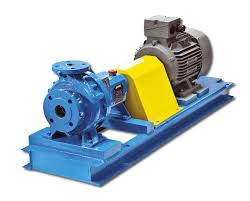
\includegraphics[width=0.4\textwidth]{pump1.jpg}
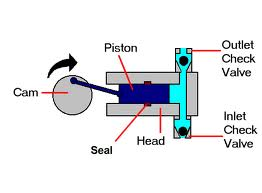
\includegraphics[width=0.45\textwidth]{rec_pump1.jpg}
\caption{\label{fig:pumps}Two examples of pumps: (left) centrifugal pump (right) positive displacement pump (piston pump)}
\end{center}
\end{figure}

Mechanical pumps serve in a wide range of applications such as pumping water from wells, aquarium filtering, pond filtering and aeration, in the car industry for water-cooling and fuel injection, in the energy industry for pumping oil and natural gas or for operating cooling towers. In the medical industry, pumps are used for biochemical processes in developing and manufacturing medicine, and as artificial replacements for body parts, e.g. the artificial heart.

The two most important quantities characterizing a pump are the pressure difference between the suction and pressure side of the pump $\Delta p$ and the flow rate delivered by the pump $Q$. For practical reasons, in the case of water technology, the \emph{pressure head} is usually used, which is pressure given in meters of fluid column: $H=\frac{\Delta p}{\rho g}$. Simple calculations reveals that for water 1 bar ($10^5\mathrm{Pa}$) pressure is equivalent of 10 mwc (meters of water column).

\subsubsection{Turbopumps}

In the case of a turbopump, a rotating impeller adds energy to the fluid. The head is computed with the help of Euler's turbine equation
%
\begin{equation}
H = \left.\frac{c_{\mathrm{2u}}u_\mathrm{2}-c_{\mathrm{1u}}u_\mathrm{1}}{g}\right|_{c_{1u=0}} =\frac{c_{\mathrm{2u}}u_\mathrm{2}}{g}
\end{equation}
%
\noindent while the flow rate is 
%
\begin{equation}
Q = D_2 \pi b_2 c_{\mathrm{2m}},
\end{equation}
%
with $c_{2u}$ and $c_{1u}$ being the circumferential component of the absolute velocity at the outlet and inlet, respectively, $u_1=D_1 \pi n$ and $u_2=D_2 \pi n$ the circumferential velocities. $c_{2m}$ stands for the radial (meridian) component of the absolute velocity at the outlet, $D$ is diameter and $b$ stand for the width of the impeller. (See Figure \ref{fig:vel_triang} and \emph{Fluid Machinery} lecture notes for further details.)

\begin{figure}[h]
\begin{center}
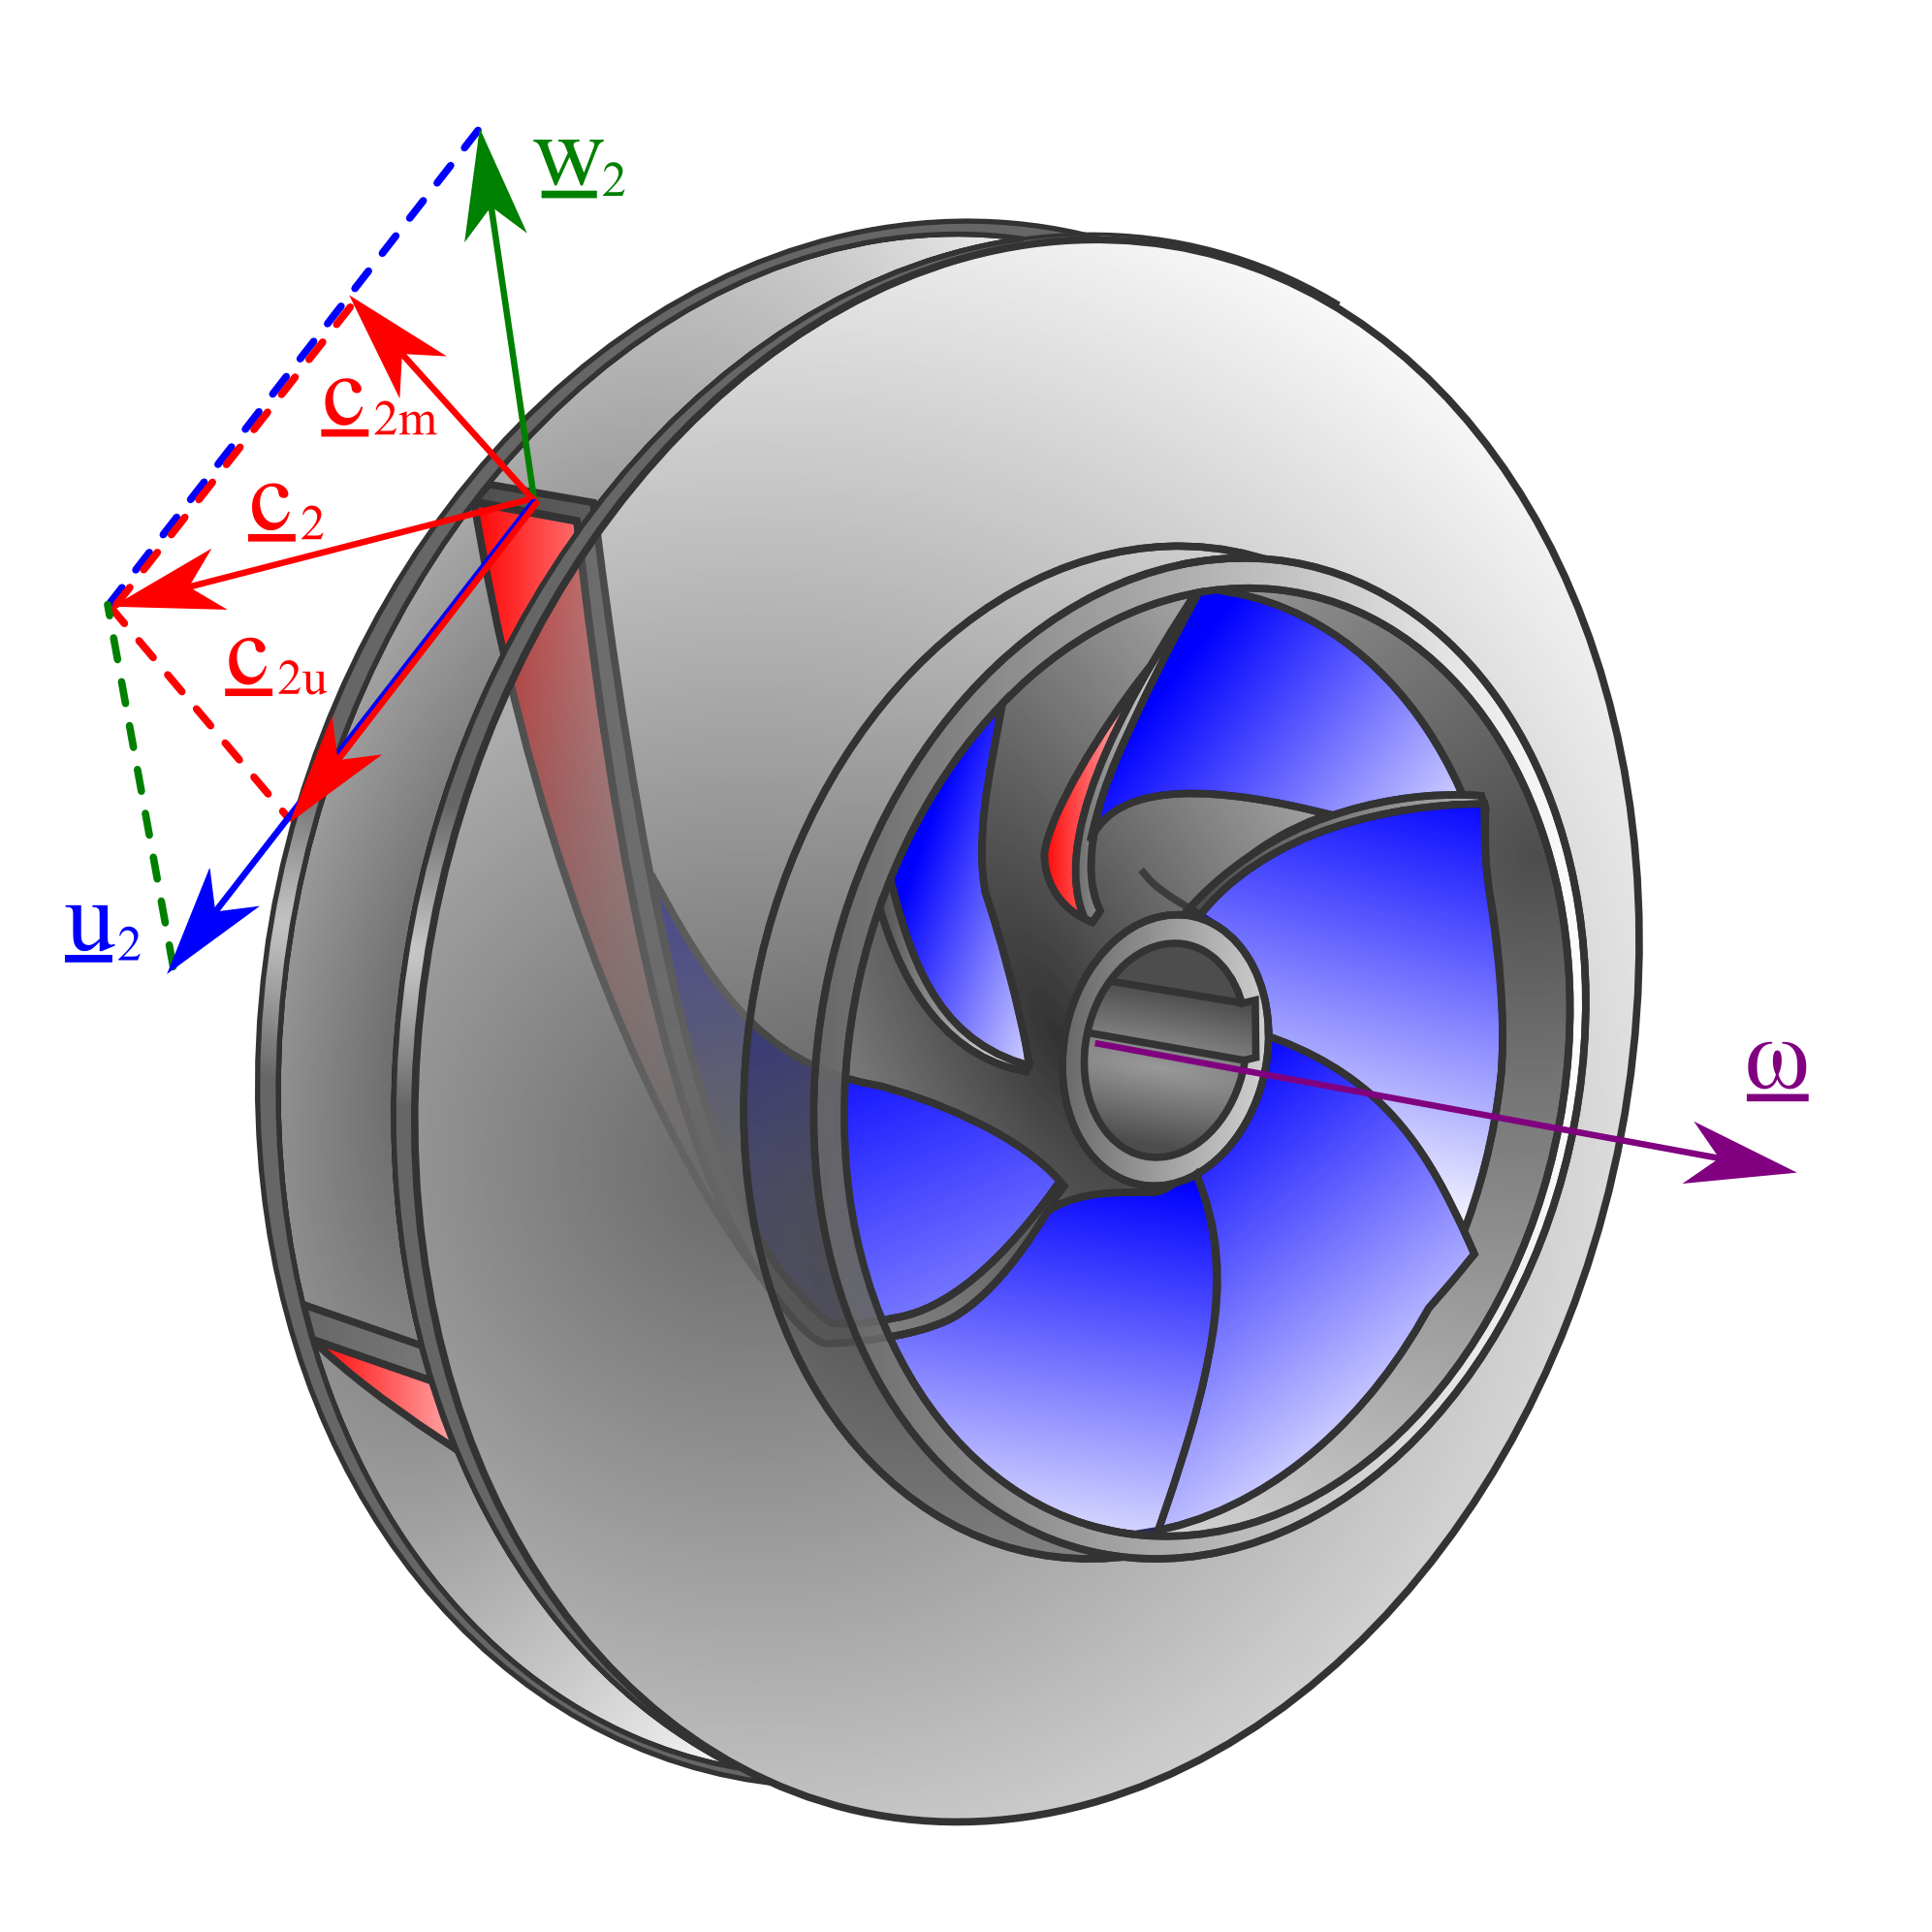
\includegraphics[width=0.4\textwidth]{Impeller3D_and_VelocityTriangles.png}
\caption{\label{fig:vel_triang}Velocity triangles on a centrifugal impeller.}
\end{center}
\end{figure}

Notice that the head ($H$) and flow rate ($Q$) are provided by the two component of the same velocity vector $c_2$. Thus, if $H$ increases, $Q$ decreases and vice versa. Thus \emph{in the case of turbomachines the pressure difference and the flow rate are directly connected and not independent.} This dependency is described by the pump's performance curve, see Figure \ref{fig:turbopump_perf_curve}.

\begin{figure}[th]
\begin{center}
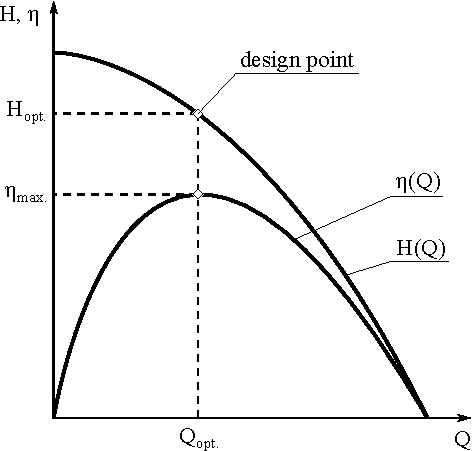
\includegraphics[scale=0.8]{lecture1_fig01_QH.pdf}
\caption{\label{fig:turbopump_perf_curve}Turbopump performance curves}
\end{center}
\end{figure}

An important quantity describing the shape of the impeller of a turbopump is the specific speed $n_q$, defined as
%
\begin{equation}
n_q=n\,\frac{Q^{1/2}_{\mathrm{opt.}}}{H^{3/4}_{\mathrm{opt.}}}\quad \mathrm{[rpm]}\,\frac{\mathrm{[m^3/s]^{1/2}}}{\mathrm{[m]^{3/4}}}.
\end{equation}
%
The dimension (unit) of $n_q$ is not emphasised and mostly omitted. The concept of specific speed can be used to determine the pump type (i.e. radial/mixed/axial) which is capable of performing a pumping problem efficiently.

\begin{figure}[h!]
\begin{center}
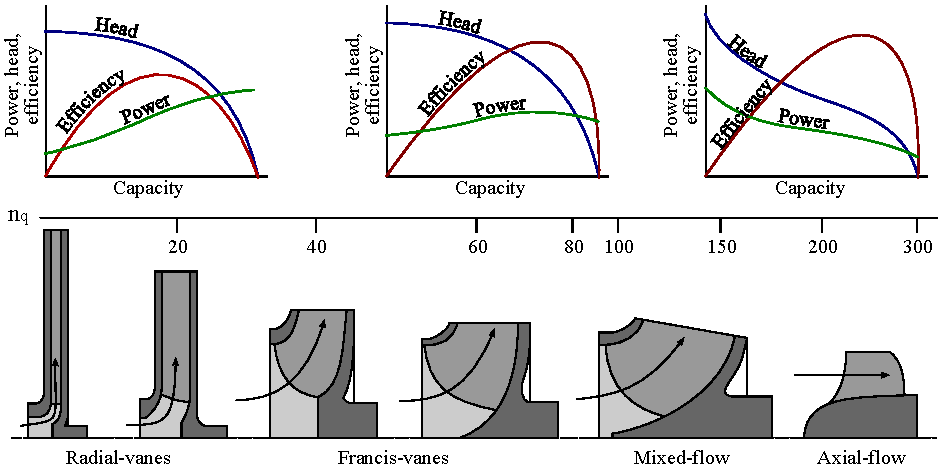
\includegraphics[scale=0.8]{nq.pdf}
\caption{\label{fig:nq}Turbopump performance curves}
\end{center}
\end{figure}

%%%%%%%%%%%%

\vspace{0.5cm}

\noindent {\bf Example 1.} We have to pump clean water to an upper reservoir at 60 m height. The nominal power of the driving electric motor is 5 kW, its revolution number is 3000 rpm. The flow rate is (assuming 100\% efficiency)
%
\begin{equation}
P_{\mathrm{motor}}=\Delta p\cdot Q\rightarrow Q=\frac{P_{\mathrm{motor}}}{\Delta p}=\frac{P_{\mathrm{motor}}}{\rho gH}=8.49\times 10^{-3}\,\mathrm{m^3/s}=509\,\mathrm{l/min}
\end{equation}
%
\noindent Hence the specific speed is
%
\begin{equation}
n_q=n\,\frac{Q^{1/2}_{\mathrm{opt.}}}{H^{3/4}_{\mathrm{opt.}}}=3000\frac{\left(8.49\times 10^{-3}\right)^{1/2}}{\left(60\right)^{3/4}}\cong 12.8,
\end{equation}
%
\noindent which means that a centrifugal turbopump is suitable for this problem.

%%%%%%%%%%%%

\vspace{0.5cm}

\noindent {\bf Example 2.} Now consider the hydraulic cylinder depicted in Figure \ref{fig:hydraulic_cylinder}. The required pressure difference is now $\Delta p=200 \mathrm{bar} = 2\times 10^7 \mathrm{Pa}$, the power and the revolution number of the driving motor is the same as before (5kW, 3000rpm).

\begin{figure}[tbh]
\begin{center}
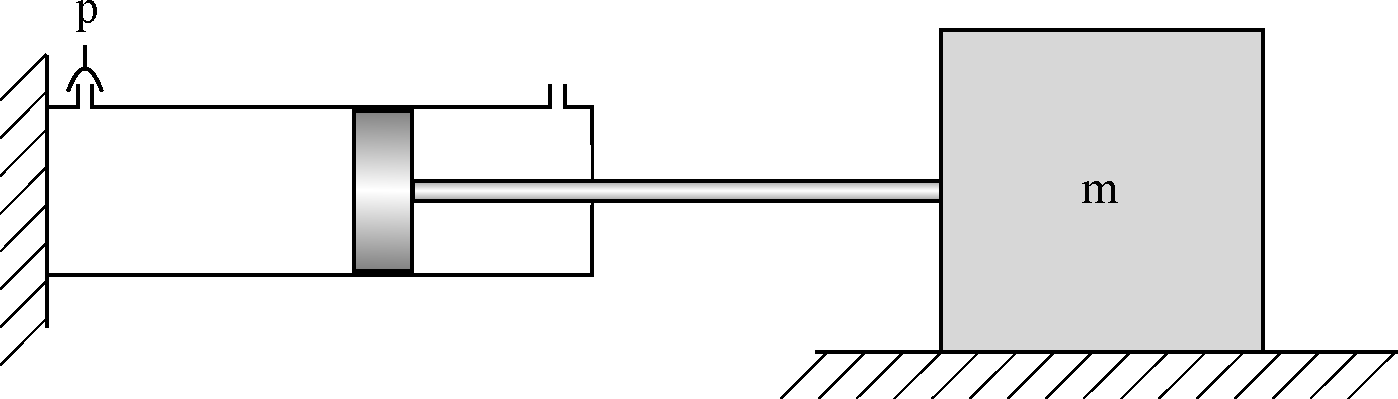
\includegraphics[width=100mm]{lecture1_fig02_dugattyu.pdf}
\caption{\label{fig:hydraulic_cylinder}Simple sketch of a hydraulic cylinder}
\end{center}
\end{figure}

\noindent First, find the flow rate of the pump (again, assume 100\% efficiency):
%
\begin{equation}
Q=\frac{P_{\mathrm{motor}}}{\rho gH}=\frac{5000}{9810\cdot 2000}=2.55\times 10^{-4}\,\mathrm{m^3/s}=15.3\,\mathrm{liter/min},
\end{equation}
%
which gives
%
\begin{equation}
n_q=n\,\frac{Q^{1/2}_{\mathrm{opt.}}}{H^{3/4}_{\mathrm{opt.}}}=3000\frac{\left(2.55\times 10^{-4}\right)^{1/2}}{\left(2000\right)^{3/4}}= 0.16.
\end{equation}
%
\noindent Comparing this value with Figure \ref{fig:nq} we see that this value is 'off' the chart. Such a small $n_q$ value would require an extremely large-diameter impeller, which is very thin. Besides the problems with the high centrifugal stresses, from the fluid mechanical point of view, such a thin impeller introduces extremely large fluid friction resulting in poor efficiency. Thus we conclude that {\bf pumping problems resulting in high pressure difference and low flow rates (i.e. $n_q< \mathrm{say,} 10$) cannot be efficiently solved by centrifugal pumps}.


\subsubsection{Positive displacement pumps}

Positive displacement pumps (PDPs) are typically used in high-pressure (above $\Delta p > 10 bar$, up to 1000-2000 bars) technology, with relatively low flow rate. These machines have an expanding cavity on the suction side and a decreasing cavity on the discharge side. Liquid flows into the pumps as the cavity on the suction side expands and the liquid flows out of the discharge as the cavity collapses. The volume is constant given each cycle of operation.

The positive displacement pumps can be divided in two main classes (see Figures XXX)
\begin{itemize}
\item reciprocating
\begin{itemize}
\item piston pumps
\item plunger pumps
\item diaphragm pumps
\item axial/radial piston pumps
\end{itemize}
\item rotary
\begin{itemize}
\item gear pumps
\item lobe pumps
\item vane pumps
\item progressive cavity pumps
\item peripheral pumps
\item screw pumps
\end{itemize}
\end{itemize}

\begin{figure}[h!]
\begin{center}
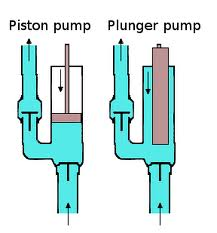
\includegraphics[width=0.3 \textwidth]{plunger_piston_pump.jpg}
\includegraphics[width=0.45 \textwidth]{axial_piston_pump.jpg}
\caption{\label{fig:reiprocating_pumps}Some reciprocating pumps}
\end{center}
\end{figure}

\begin{figure}[h!]
\begin{center}
\includegraphics[width=0.3 \textwidth]{gear_pump.jpg}
\includegraphics[width=0.3 \textwidth]{vane_pump.jpg}
\includegraphics[width=0.3 \textwidth]{double-screw_pump.jpg}
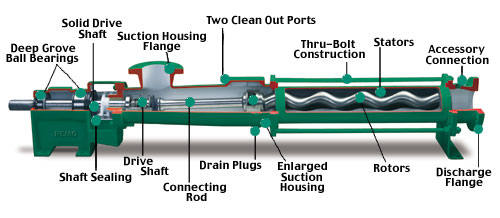
\includegraphics[width=0.6 \textwidth]{progressive_cavity_pump.jpg}
\caption{\label{fig:reiprocating_pumps}Some rotary pumps}
\end{center}
\end{figure}

PDPs, unlike a centrifugal pumps, will produce the same flow at a given motor speed (rpm) no matter the discharge pressure, hence PDPs are \emph{constant flow machines}. A PDP must not be operated against a closed valve on the discharge (pressure) side of the pump because it has no shut-off head like centrifugal pumps: a PDP operating against a closed discharge valve will continue to produce flow until the pressure in the discharge line are increased until the line bursts or the pump is severely damaged - or both.

A relief or safety valve on the discharge side of the PDP is therefore absolute necessary. The relief valve can be internal or external. The pump manufacturer has normally the option to supply internal relief or safety valves. The internal valve should in general only be used as a safety precaution, an external relief valve installed in the discharge line with a return line back to the suction line or supply tank is recommended.

Several types of PDPs can be used as motors: if fluid is driven through them (e.g. gear pump), the shaft rotates and the same machine can be used as a motor.

\clearpage

\subsection{Basic characteristics of positive displacement machines}

The pump \emph{displacement} $V_g$ is the volume of the liquid delivered by the pump per one revolution, assuming no leakage (zero pressure difference between the suction and pressure side) and neglecting the fluid compressibility. The \emph{ideal -- theoretical -- flow rate} is
%
\begin{equation}
Q_{th}=n V_g
\label{eq:Qth}
\end{equation}
%
where $Q_{th}$ is theoretical flow rate ($\mathrm{liter/min})$, $n$ is the revolution number of the pump shaft ($\mathrm{rpm}$) and $V_g$ stands for the pump displacement, ($\mathrm{cm^3}$). 

In the case of {\bf pumps}, the actual outflow is less than the theoretical flow rate, due to the leakages inside the pump. These losses are taken into by the \emph{volumetric efficiency} $\eta_{vol}$: $Q=\eta_{\mathrm{vol}} Q_{\mathrm{th}} = \eta_{\mathrm{vol}}\, n\,  V_{\mathrm{g}}$. Other types of losses (sealing, bearing, fluid internal and wall friction) are all concentrated into the so-called \emph{hydromechanical efficiency} $\eta_{hm}$, which connects the input and output power: $P_{in} \eta_{hm}=P_{out}$. For pumps, $P_{in}=M \omega$ and $P_{out}=Q \Delta p$. We have:
%
\begin{equation}
\eta_{hm} \underbrace{M \underbrace{2\pi n}_{\omega}}_{P_{in}}=\underbrace{\underbrace{n V_g \eta_{vol}}_Q\Delta p}_{P_{out}}
\quad \rightarrow \quad
\Delta p_{pump}=\frac{2\pi M}{V_{\mathrm{g}}}\frac{\eta_{hm}}{\eta_{vol}}
\end{equation}

In the case of {\bf motors}, the input power is hydraulic power ($P_{in}=Q \Delta p$) and the output is rotating mechanical power $P_{out}=M \omega$. Due to the internal leakage, one has to 'push' more fluid into the pump to experience the same revolution number, hence $Q=Q_{th}/\eta_{vol}>Q_{th}$. We have:
%
\begin{equation}
\eta_{hm} 
\underbrace{
\underbrace{
\frac{n V_g}{\eta_{vol}}
}_Q
\Delta p}_{P_{in}}=\underbrace{M \underbrace{2\pi n}_{\omega}}_{P_{out}}
\quad \rightarrow \quad
\Delta p_{motor}=\frac{2\pi M}{V_{\mathrm{g}}}\frac{\eta_{vol}}{\eta_{hm}}
\end{equation}

\begin{figure}[ht]
\begin{center}
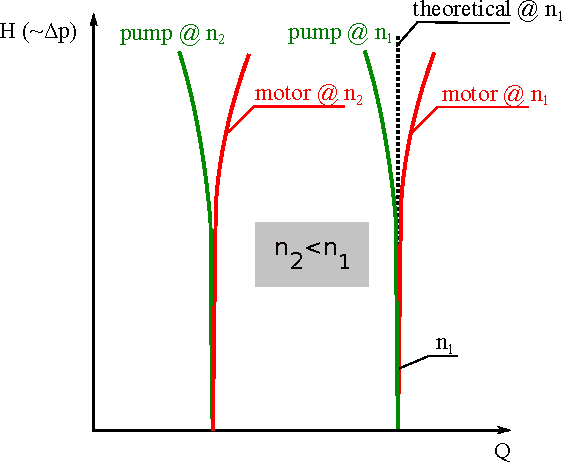
\includegraphics[width=0.5 \textwidth]{motor_pump_perf_curve_QH.pdf}
\caption{\label{fig:pump_and_motor_perf_curve}Pump and motor performance curves for two different revolution mubers.}
\end{center}
\end{figure}

\noindent We conclude that for both pumps and motors,

\begin{equation}
\shadowbox{$\displaystyle
Q \propto n,V_g \quad \text{and} \quad \Delta p \propto M,\frac{1}{V_g}.
$}
\end{equation}

\noindent Which means that the pressure and the flow rate are independent for a given machine. The same behaviour can be observed on the performances curve of these machines, see Figure \ref{fig:pump_and_motor_perf_curve}. The theoetical performance lines are vertical for a given revolution speed, meaning that the theoretical flow rate does not change when varying the pressure.

However, the leakage flow rate through the small internal gaps of the pumps (motors) slighty change ths theoretical behaviour. In the case of pumps, a portion of the flow rate flows back from the pressure side to the suction side through these gaps, hence reducing the outflow of the pump. The higher the pressure difference is, the higher the leakage flow rate is, hence the pump performance curves tend to `bend to the left' from the vertical, theoretical line. In the case of motors, where the fluid drives the shaft, we need larger flow rates to reach the desired revolution number, hence the real curves `bend to the right'.

\clearpage

\section{Reciprocating Pumps}

Piston/plunger pumps comprise of a cylinder with a reciprocating piston/plunger in it. In the head of the cylinder the suction and discharge valves are mounted. In the suction stroke the plunger retracts and the suction valves opens causing suction of fluid into the cylinder. In the forward stroke the plunger push the liquid out the discharge valve.

With only one cylinder the fluid flow varies between maximum flow when the plunger moves through the middle positions, and zero flow when the plunger is in the end positions. A lot of energy is wasted when the fluid is accelerated in the piping system. Vibration and "water hammers" may be a serious problem. In general the problems are compensated by using two or more cylinders not working in phase with each other.

Several cylinders can be mounted to the same shaft: pumps with 1 cylinder are called \emph{simplex} pumps, \emph{duplex} pumps have two cylinders (with $\pi$ phase shift) while \emph{triplex} pumps have three pumps with $2 \pi/3 = 120$ degrees phase shift. Pumps with even more pistons (5,7,9) are also common. Pumps with both sides of the piston acting (deing in contact with the liquied) are called \emph{double-acting} pumps.


\subsection{Single-acting piston pumps}




\begin{figure}[tbh]
\begin{center}
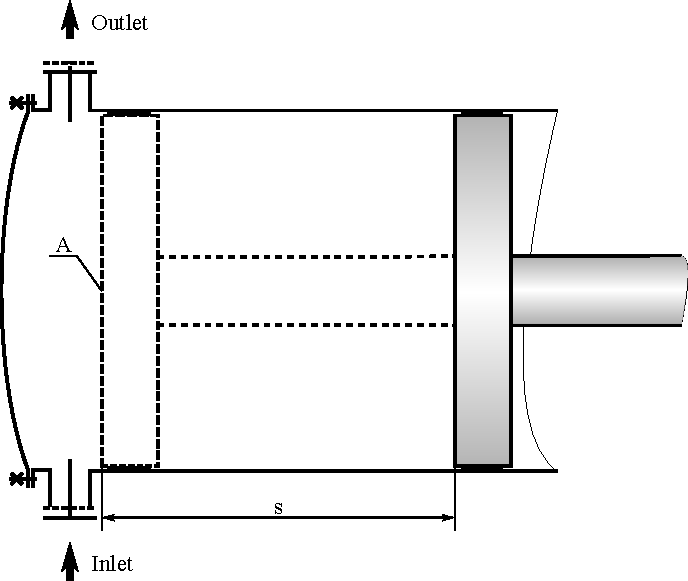
\includegraphics[scale=0.7]{lecture2_fig10_dugattyus_szivattyu.pdf}
\caption{\label{fig:single_acting_piston_pump}Single-acting piston pump}
\end{center}
\end{figure}

Consider the piston pump depicted in Figure \ref{fig:single_acting_piston_pump}.  First, let us find the $x(t)$ displacement of the piston as a function of time. By virtue of the cosine law, we have
%
\begin{equation}
L^2=R^2+y(t)^2- 2 R y(t) \cos \varphi \quad \rightarrow \quad y(t)=R \cos \varphi \pm \sqrt{L^2+R^2\left( 1-\cos^2 \varphi\right)}
\end{equation}
%
with $\varphi=\omega t$. Notice that if $\varphi=0$, we must have $y(0)=R+L$, hence we need the 'plus' case in the above equation. The piston displacement is 
%
\begin{equation}
x(t)=y(t)-y(\pi)=R \left( 1+ \cos \varphi  - \lambda^{-1} \left(
1- \sqrt{1+\lambda^2\left( 1-\cos^2 \varphi\right)}
\right)\right),
\end{equation}
%
with $\lambda=R/L$. Now consider the terms in the bracket. First, $1+\cos \varphi$ varies between 0 and 2. The second term varies between 0 ($\cos \varphi=\pm1$) and $\lambda^{-1} \left(1- \sqrt{1+\lambda^2} \right)$ ($\cos \varphi=0$), which gives $0.2361$, $0.099$ and $0.0499$ for $\lambda=R/L=1/2,1/5$ and $1/10$, respectively. Hence we conclude that if $\lambda<0.2$ (which s trus for many real-life configurations), the error due to neglecting the $\lambda^{-1}(\dots)$ term is less than 10\%, which is acceptable.

Hence we approximate the piston displacement as
%
\begin{equation}
x(t)\approx R\left(1+\cos \left( \omega t\right) \right), \quad 
v(t)\approx-R \omega \sin \left( \omega t\right) \quad \text{and} \quad 
a(t)\approx-R \omega^2 \cos \left( \omega t\right).
\end{equation}
%
As flow rate is $Q=Av$ and the stroke is $s=2R$, the \emph{instantaneous} pressure side flow rate is (see also Figure \ref{fig:single_acting_piston_pump_curves})
%
\begin{equation}
Q(t)=
\begin{cases}
A\frac{s}{2}\omega\cos(\omega t) & \mathrm{if} \quad  \pi < \varphi=\omega t < 2 \pi \\
0 & \mathrm{if}\quad  0 < \varphi=\omega t < \pi
\end{cases}
\label{eq:single_piston_pump_flowrate}
\end{equation}
% \begin{equation}
% Q(t)=A\underbrace{v(t)}_{\frac{\mathrm{d}}{\mathrm{d}t}x(t)}=A\frac{s}{2}\omega\cos(\omega t).
% \label{eq:single_piston_pump_flowrate}
% \end{equation}
%
The mean flow rate is computed by finding the volume of the fluid pushed to the pressure side in one period, divided by the length of the period:
%
\begin{equation}
Q_{mean} = A s n, 
\end{equation}
%
that is, we have $V_g = A s$, see \eqref{eq:Qth}. The maximum flow rate is (see \eqref{eq:single_piston_pump_flowrate})
%
\begin{equation}
Q_{max} = A \frac{s}{2} \omega= \pi A s n = \pi Q_{mean}. 
\end{equation}

\begin{figure}[th]
\begin{center}
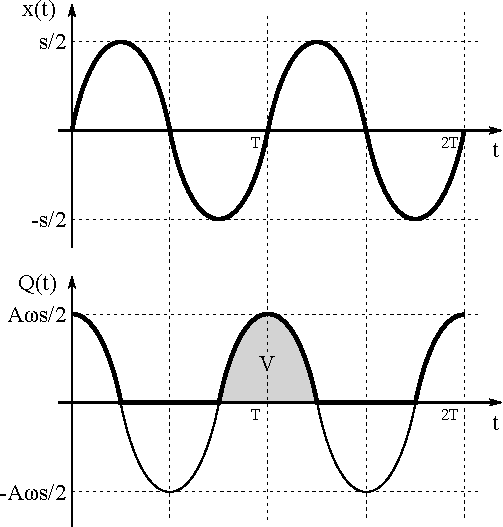
\includegraphics[width=0.5\textwidth]{lecture2_fig11_dugattyus_szivattyu_diagram.pdf}
\caption{\label{fig:single_acting_piston_pump_curves} Piston displacement (upper panel) and flow rate ($\propto$ velocity) curves of a single-acting piston pump.}
\end{center}
\end{figure}

Notice that this means that these pumps induce an extremely unsteady flow rate in the pipeline system, that varies from $Q_{min}=0$ flow rate up to $Q_{max}=\pi Q_{mean}$ with a frequency of $n$ (driving motor revolution number). There are two ways of reducing this pulsation: (a) by using multiple pistons or (b) adding a pulsation damper.

\clearpage

\subsection{Multiple piston pumps}

The pulsation can be reduced by adding several pistons with an evenly distributed phase shift, see e.g. Figure \ref{fig:double_acting_piston_pump}. 

\begin{figure}[th]
\begin{center}
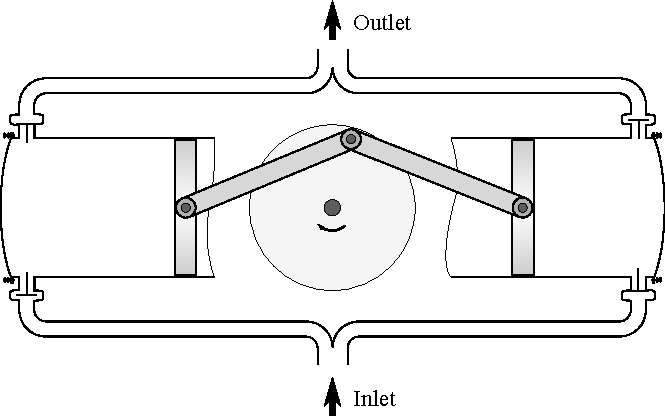
\includegraphics[scale=0.9]{lecture2_fig12_duplex_dugattyus_szivattyu.pdf}
\caption{\label{fig:double_acting_piston_pump}Double-acting piston pump}
\end{center}
\end{figure}

\noindent If we have three pistons (triplex), the flow rates are 
%
\begin{align*}
Q_1(t) &= \text{max}(0, A s n \pi\cos(\omega t))\\
Q_2(t) &= \text{max}(0, A s n \pi\cos(\omega t-\frac{2\pi}{3}))\quad \text{and}\\
Q_3(t) &= \text{max}(0, A s n \pi\cos(\omega t-2 \times\frac{2\pi}{3})).
\end{align*}
%
The overall flow rate is $Q(t)=Q_1(t)+Q_2(t)+Q_3(t)$. Let us define the \emph{pulsation factor} measuring the relative flow rate change as
%
\begin{equation}
\delta =\frac{Q_{\mathrm{max}}-Q_{\mathrm{min}}}{Q_{\mathrm{mean}}}\,[\%].
\end{equation}
%
For example, for a single-acting pump we have
\begin{equation}
\delta =\frac{Q_{\mathrm{max}}-Q_{\mathrm{min}}}{Q_{\mathrm{mean}}}=\frac{\pi Q_{\mathrm{mean}}-0}{Q_{\mathrm{mean}}}=\pi = 314\,\%
\end{equation}

\begin{figure}[ht]
\begin{center}
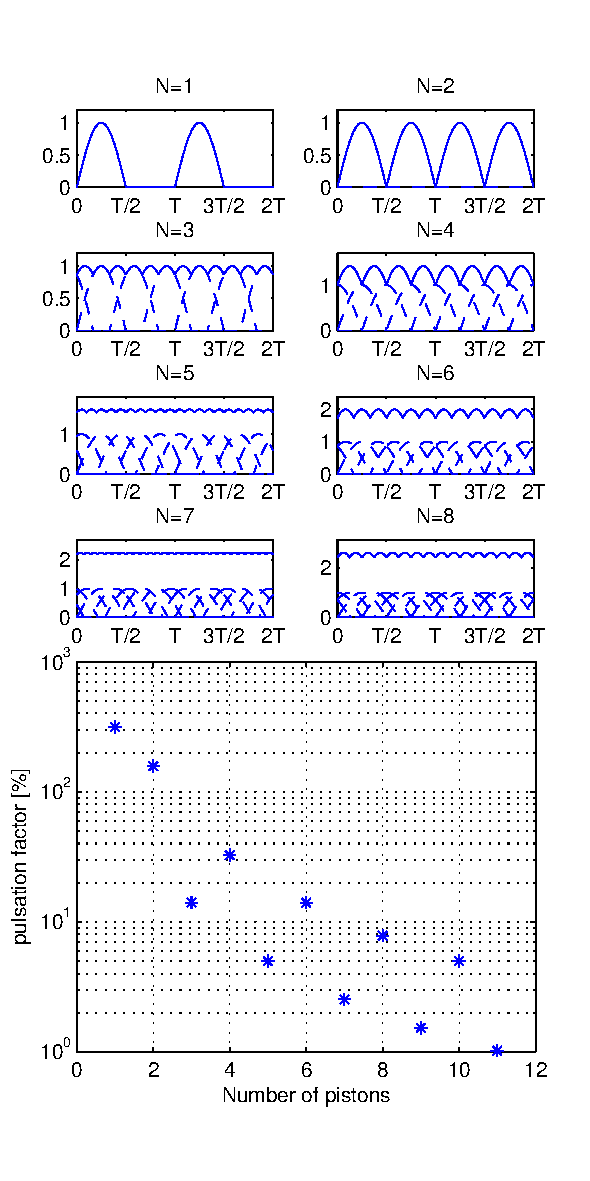
\includegraphics[width=12cm]{piston_pump_pulsation_factor.pdf}
\caption{\label{fig:pulsation_factor}Pulsation factor as a function of the piston number.}
\end{center}
\end{figure}

Similar calculation for other number of pistons gives the values in Table \ref{tab:piston_puls}. Figure \ref{fig:pulsation_factor} depicts the flow rate for several numbers of pistons, where dashed lines are the individual flow rates while solid lines are the pump flow rate (sum of the piston flow rates) and the pulsation factor as a function of the piston number. Notice that if the number of pistons is odd (e.g. 3,5,7,9), the pulsation number is significantly lower.

\begin{table}[h]
\centering
\begin{tabular}{l||c|c|c|c|c|c|}
Number of pistons & 1 & 2 & 3 & 4 & 5 & 9\\ \hline
$\delta $ \%      &  315 & 157 & 14 & 33 & 5 & 1.5
\end{tabular}
\caption{\label{tab:piston_puls}Flow rate pulsation level as a function of the piston number.}
\end{table}
\clearpage

%%%%%%%%%%%%%%%%%%%%%%%%%%%%%%%%%%%%%%%%%%%%%%%%%%%%
\subsection{Axial piston pumps}

An axial piston pump is a positive displacement pump that has a number of pistons in a \emph{circular array} within a cylinder block. It can be used as a stand-alone pump, a hydraulic motor or an automotive air conditioning compressor. Axial piston pumps are used to power the hydraulic systems of jet aircrafts, being gear-driven off of the turbine engine's main shaft. The system used on the F-14 used a 9-piston pump that produced a standard system operating pressure of 3000 psi and a maximum flow of 84 gallons per minute.  Advantages:

\begin{itemize}
\item high efficiency
\item  high pressure (up to 1,000 bar)
\item  low flow and pressure ripple (due to the small dead volume in the workspace of the pumping piston)
\item low noise level
\item high reliability
\end{itemize}


Axial piston units are available in the form of pumps and motors in bent axis design or swashplate design for medium- and high-pressure ranges. They are the main components in the hydrostatic transmission. Compact size and high power density, economy and reliability are characteristic advantages which speak for the use of hydrostatic transmissions, together with the fact that they meet the demand for high speed and high torque, as well as optimum efficiency. 

\begin{figure}[h!]
\begin{center}
\includegraphics[height=5cm]{figs/axial_piston_pump.jpg}
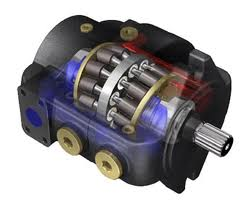
\includegraphics[height=5cm]{figs/axial_piston_pump_cutaway.jpg}
\caption{\label{fig:ax_pp} Axial piston pump}
\end{center}
\end{figure}

%%%%%%%%%%%%%%%%%%%%%%%%%%%%%%%%%%%%%%%%%%%%%%%%%%%%
\subsection{Radial piston pumps}

In a radial piston pump the working pistons extend in a radial direction symmetrically around the drive shaft, in contrast to the axial piston pump. These kinds of piston pumps are characterized by the following advantages:
\begin{itemize}
\item high efficiency
\item  high pressure (up to 1,000 bar)
\item  low flow and pressure ripple (due to the small dead volume in the workspace of the pumping piston)
\item low noise level
\item very high load at lowest speed due to the hydrostatically balanced parts possible
\item no axial internal forces at the drive shaft bearing
\item high reliability
\end{itemize}

A disadvantage are the bigger radial dimensions in comparison to the axial piston pump, but it could be compensated with the shorter construction in axial direction.

Due to the hydrostatically balanced parts it is possible to use the pump with various hydraulic fluids like mineral oil, biodegradable oil, HFA (oil in water), HFC (water-glycol), HFD (synthetic ester) or cutting emulsion. That implies the following main applications for a radial piston pump:
machine tools (e.g., displace of cutting emulsion, supply for hydraulic equipment like cylinders)
\begin{itemize}
\item high pressure units (HPU) (e.g., for overload protection of presses)
\item test rigs
\item automotive sector (e.g., automatic transmission, hydraulic suspension control in upper-class cars)
\item plastic- and powder injection moulding
\item wind energy
\end{itemize}

\begin{figure}[h!]
\begin{center}
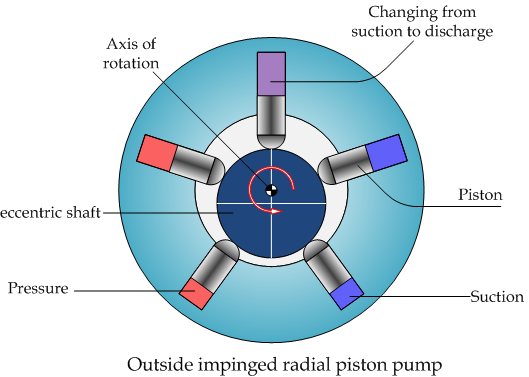
\includegraphics[height=5cm]{figs/radial_piston_pump1.png}
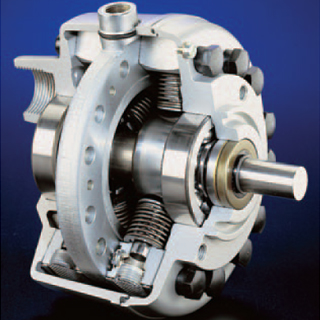
\includegraphics[height=5cm]{figs/radial_piston_pump_cutaway.jpg}
\caption{\label{fig:rad_pp} Radial piston pump}
\end{center}
\end{figure}

%%%%%%%%%%%%%%%%%%%%%%%%%%%%%%%%%%%%%%%%%%%%%%%%%%%%
\subsection{Diaphragm pumps}

A diaphragm pump (also known as a membrane pump) is a positive displacement pump that uses a combination of the reciprocating action of a rubber, thermoplastic or teflon diaphragm and suitable valves either side of the diaphragm (check valve, butterfly valves, flap valves, or any other form of shut-off valves) to pump a fluid. The advantages of these pumps are:
\begin{itemize}
\item They provide \emph{leakage-free sealing}, which can be important when pumping highly aggressive or toxic fluids.
\item They have good suction lift characteristics, some are low pressure pumps with low flow rates; others are capable of higher flow rates, dependent on the effective working diameter of the diaphragm and its stroke length. 
\item They can handle sludges and slurries with a relatively high amount of grit and solid content.
\item Suitable for discharge pressure up to 1200 bar
\item They have good dry running characteristics.
% \item can be used to make artificial hearts.
% are used to make air pumps for the filters on small fish tanks.
\item Good efficiency (can be up to 97\%)
\item Can handle highly viscous liquids.
\end{itemize}

However, as they are single (or sometimes double-acting) piston pumps, these pumps cause a pulsating flow that may cause water hammer, which can be minimised by using a pulsation dampener.

\begin{figure}[h!]
\begin{center}
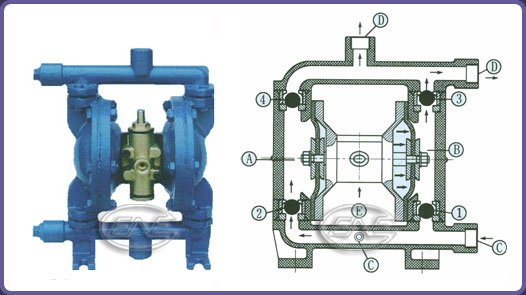
\includegraphics[width=\textwidth]{figs/diaphragmpump61_1.jpg}
% 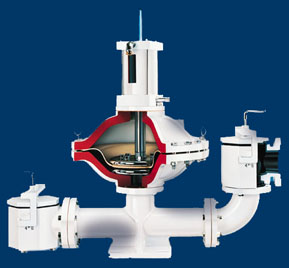
\includegraphics[height=5cm]{figs/gr-addcutaway.jpg}
\caption{\label{fig:diap_pp} Diaphragm pump}
\end{center}
\end{figure}

\clearpage

%%%%%%%%%%%%%%%%%%%%%%%%%%%%%%%%%%%%%%%%%%%%%%%%%%%%%%%%%%%%%%%%%%%%%%%%%%%%%%%%%%%%%%%%%%%%%%%%%%

\section{Rotary pumps}

\subsection{Gear pumps}
This is the simplest of rotary positive displacement pumps consisting of two meshed gears rotating in a closely fitted casing. Fluid is pumped around the outer periphery by being trapped in the tooth spaces. It does not travel back on the meshed part, since the teeth mesh closely in the centre. It is widely used on car engine oil pumps, and also in various hydraulic power packs.

There are two main variations; external gear pumps which use two external spur gears, and internal gear pumps which use an external and an internal spur gear. Some gear pumps are designed to function as either a motor or a pump.

\begin{figure}[h!]
\begin{center}
\includegraphics[height=4cm]{figs/gear_pump.jpg}
\hspace{1cm}
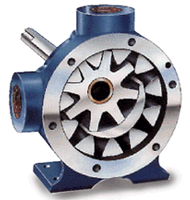
\includegraphics[height=5cm]{figs/genpur.png}
\caption{\label{fig:gear_pumps} (left) external gear pump (right) internal gear pump}
\end{center}
\end{figure}

\subsubsection{External gear pumps}

\noindent Advantages:
\begin{itemize}
\item High speed
\item High pressure
% \item No overhung bearing loads
\item Relatively quiet operation
\end{itemize}

\noindent Disadvantages:
\begin{itemize}
\item Four bushings in liquid area
\item No solids allowed
\item Fixed end clearances
\end{itemize}

\noindent Common external gear pump applications include, but are not limited to:
\begin{itemize}
\item Various fuel oils and lube oils
\item Chemical additive and polymer metering
\item Chemical mixing and blending (double pump)
\item Industrial and mobile hydraulic applications (log splitters, lifts, etc.)
\item Acids and caustic (stainless steel or composite construction)
% \item Low volume transfer or application
\end{itemize}

\subsubsection{Internal gear pumps}

\noindent Advantages:
\begin{itemize}
\item Only two moving parts
\item Only one stuffing box
\item Non-pulsating discharge
\item Excellent for high-viscosity liquids
% \item Constant and even discharge regardless of pressure conditions
\item Operates well in either directions
% \item Can be made to operate with one direction of flow with either rotation
\item Low NPSH required
\item Single adjustable end clearance
\item Easy to maintain
% \item Flexible design offers application customization
\end{itemize}

\noindent Disadvantages:
\begin{itemize}
\item Usually requires moderate speeds
\item Medium pressure limitations
\item One bearing runs in the product pumped
% \item Overhung load on shaft bearing
\end{itemize} 

\noindent Common internal gear pump applications include, but are not limited to:
\begin{itemize}
\item All varieties of fuel oil and lube oil
\item Resins and polymers
\item Alcohols and solvents
\item Asphalt, bitumen, and tar
% \item Polyurethane foam (Isocyanate and polyol)
\item Food products such as corn syrup, chocolate, and peanut butter
\item Paint, inks, and pigments
\item Soaps and surfactants
\item Glycol
\end{itemize}


\subsection{Screw pump}
Screw pumps feature two or three screws with opposing thread, that is, one screw turns clockwise, and the other counterclockwise. The screws are each mounted on shafts that run parallel to each other; the shafts also have gears on them that mesh with each other in order to turn the shafts together and keep everything in place. The turning of the screws, and consequently the shafts to which they are mounted, draws the fluid through the pump. As with other forms of rotary pumps, the clearance between moving parts and the pump's casing is minimal.


\begin{figure}[h!]
\begin{center}
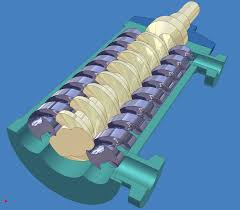
\includegraphics[height=4cm]{figs/simple_screw_pump.jpg}
\hspace{1cm}
\includegraphics[height=5cm]{figs/double-screw_pump.jpg}
\caption{\label{fig:screw_pumps} (left) simple screw pump (right) double-screw pump used for pumping crude oil}
\end{center}
\end{figure}

\noindent Advantages:
\begin{itemize}
\item Practically pulsation-free flow
\item low fluid velocities $\rightarrow$ not sensitive for e.g. sand content
\end{itemize}

\noindent Disadvantages:
\begin{itemize}
\item Expensive
\end{itemize} 

\subsection{Vane pump}

\noindent Advantages:
\begin{itemize}
\item Handles thin liquids at relatively higher pressures
% \item Compensates for wear through vane extension
\item Sometimes preferred for solvents, LPG
\item Can run dry for short periods
% \item Can have one seal or stuffing box
\item Develops good vacuum
\end{itemize}

\noindent Disadvantages:
\begin{itemize}
% \item Can have two stuffing boxes
% \item Complex housing and many parts
\item Not suitable for high pressures
\item Not suitable for high viscosity
\item Not good with abrasives
\end{itemize} 

\noindent Applications:
\begin{itemize}
\item Aerosol and Propellants
\item Aviation Service - Fuel Transfer, Deicing
\item Auto Industry - Fuels, Lubes, Refrigeration Coolants
\item Bulk Transfer of LPG and NH3
\item LPG Cylinder Filling
\item Alcohols
\item Refrigeration - Freons, Ammonia
\end{itemize}

\begin{figure}[ht]
\begin{center}
\includegraphics[height=6cm]{figs/vane_pump.jpg}
\caption{\label{fig:vane_pump} Vane pump}
\end{center}
\end{figure}


\subsection{Progressing cavity pump (eccentric screw pump)}

Widely used for pumping difficult materials such as sewage sludge contaminated with large particles, this pump consists of a helical shaped rotor, about ten times as long as its width. This can be visualized as a central core of diameter x, with typically a curved spiral wound around of thickness half x, although of course in reality it is made from one casting. This shaft fits inside a heavy duty rubber sleeve, of wall thickness typically x also. As the shaft rotates, fluid is gradually forced up the rubber sleeve. Such pumps can develop very high pressure at quite low volumes.

\begin{figure}[h!]
\begin{center}
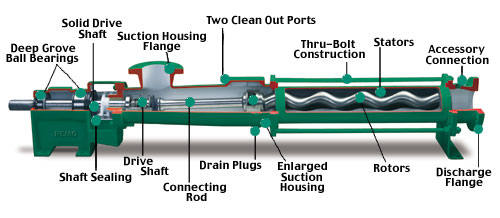
\includegraphics[width=0.7 \textwidth]{figs/cutawaylabel.jpg}
\caption{\label{fig:prog_cav_pumps} Progressive cavity pump.}
\end{center}
\end{figure}


% \frame{\frametitle{Roots-type pumps}
% Named after the Roots brothers who designed and invented it, this lobe pump works by displacing the liquid trapped between two long helical twisted rotors, each fitting into the other when perpendicular at 90°, rotating inside a triangular shaped sealing line configuration, both at the point of suction and at the point of discharge.

% This design produces a continuous flow with equal volume and no vortex. It can work at low pulsation rates and results with gentle performance, more fit for some applications.

% Some applications are:high capacity industrial air compressors, Roots Type Superchargers on internal combustion engines.
% }

\subsection{Peristaltic pump}

A peristaltic pump is a type of positive displacement pump used for pumping a variety of fluids. The fluid is contained within a flexible tube fitted inside a circular pump casing (though linear peristaltic pumps have been made). A rotor with a number of "rollers", "shoes" or "wipers" attached to the external circumference compresses the flexible tube. As the rotor turns, the part of the tube under compression closes (or "occludes") thus forcing the fluid to be pumped to move through the tube. Additionally, as the tube opens to its natural state after the passing of the cam ("restitution") fluid flow is induced to the pump. This process is called peristalsis and is used in many biological systems such as the gastrointestinal tract.

\noindent Advantages

\begin{itemize}
\item No contamination. Because the only part of the pump in contact with the fluid being pumped is the interior of the tube, it is easy to sterilize and clean the inside surfaces of the pump.
\item Low maintenance needs. Their lack of valves, seals and glands makes them comparatively inexpensive to maintain.
\item They are able to handle slurries, viscous, shear-sensitive and aggressive fluids.
\item Pump design prevents backflow and syphoning without valves.[5]
\end{itemize}

\noindent Disadvantages
\begin{itemize}
\item The flexible tubing will tend to degrade with time and require periodic replacement.
\item The flow is pulsed, particularly at low rotational speeds. Therefore, these pumps are less suitable where a smooth consistent flow is required. An alternative type of positive displacement pump should then be considered.
\end{itemize}


\begin{figure}[h!]
\begin{center}
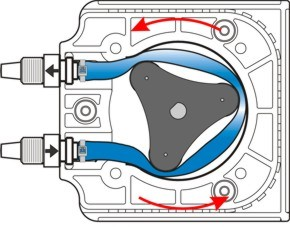
\includegraphics[width=0.4 \textwidth]{figs/per_pumphead.jpg}
\caption{\label{fig:per_pump} Peristaltic pump}
\end{center}
\end{figure}

% \frame{\frametitle{Lobe pump}
% \begin{figure}
% 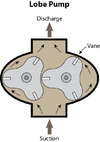
\includegraphics[scale=1]{figs/100px-Common_Lobe_Pump.png}
% \caption{Lobe pump}
% \end{figure}
% }

% \frame{\frametitle{Vane pump}
% }


%%%%%%%%%%%%%%%%%%%%%%%%%%%%%%%%%%%%%%%%%%%%%%%%%%

\clearpage

\subsection{Pulsation dampener}

A pulsation dampener is an accumulator with a set pre-charge that absorbs system shocks while minimizing pulsations, pipe vibration, water hammering and pressure fluctuations. By minimizing pulsation in the system components like regulators, solenoids, sensors, etc., pumps will see decreased wear and have longer life. Pulsation dampeners are tied directly onto the discharge manifold or plumbed immediately downstream of the pump.

\begin{figure}[h]
\begin{center}
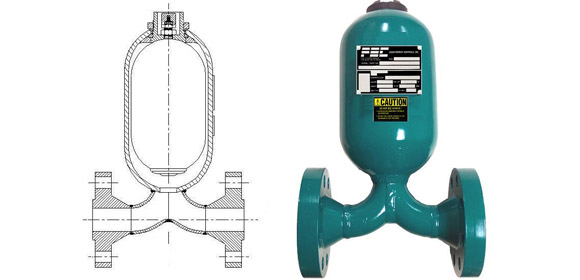
\includegraphics[width=0.8\textwidth]{pulsation_dampeners.jpg}
\caption{\label{fig:pulsation_dampener}Pulsation dampener.}
\end{center}
\end{figure}

The sizing of the dampener goes as follows. The instantaneous and mean flow rate for a single piston pump is 
%
\begin{equation}
Q(t)=Q_{max} \sin (\omega t) \quad \text{and} \quad Q_{mean}=\frac{Q_{max}}{\pi}, \quad \text{where} \quad Q_{max}=\pi A_D s n.
\label{eq:flowratepiston}
\end{equation}
%
The pump flow rate is $Q_p(t)=\sum_{i=1}^N Q_i(t)$, where $Q_i$ is the flow rate of the $i$th piston, i.e. \eqref{eq:flowratepiston} shifted with an angle of $\phi_i=(i-1)\,2\pi/N$, $N$ being the number of pistons. The average flow rate of the pump is $Q_{p,mean}=N\,Q_{mean}$.

The flow rate entering the damper is
%
\begin{equation}
Q_d(t)=Q_p(t)-Q_{p,mean},
\end{equation}
%
while the volume of fluid entering (or leaving) the damper up to time $t$ is
%
\begin{equation}
V_d(t)=\int Q_d(t) dt.
\end{equation}

In the case of a single piston, we have

\begin{align}
Q_d(t)&=\left\{
\begin{matrix}
Q_{max} \left( \sin (\omega t) -\frac{1}{\pi} \right) & \text{if} & 0\leq t \leq \frac{T}{2}\\
-Q_{max}/\pi  & \text{if} & \frac{T}{2}\leq t \leq T
\end{matrix}
\right.
%
\quad 
\text{and}\\
%
V_d(t)&=\left\{
\begin{matrix}
Q_{max} \left( -\frac{1}{\omega}\left(\cos (\omega t)-1\right) -\frac{t}{\pi}\right)  & \text{if} & 0\leq t \leq \frac{T}{2}\\
-t Q_{max} /\pi & \text{if} & \frac{T}{2}\leq t \leq T.
\end{matrix}
\right.
\end{align}

The above expression for $V_d$ also ensures that $V_d(0)=0$. Maximum and minimum volume occurs at $Q_p=0$, i.e.
%
\begin{align}
\omega t_{min}&=\arcsin \frac{1}{\pi} \quad \rightarrow \quad t_{min}=\frac{0.3239}{2 \pi}T=0.0516\,T.\\
\omega t_{max}&=\pi-\arcsin \frac{1}{\pi} \quad \rightarrow \quad t_{max}=\frac{\pi - 0.3239}{2 \pi}T=0.4484\,T.
\end{align}
%
The corresponding volumes are
\begin{equation}
V_{min}=-0.0081\,Q_{max} T=\underbrace{-0.0081 \pi}_{-0.0256} \underbrace{Q_{mean}T}_{V_{stroke}} \quad \text{and} \quad V_{min}=0.1673\,Q_{max} T =0.5256 V_{stroke},
\end{equation}
%
hence the total volume variation on the damper is
%
\begin{equation}
\Delta V=V_{max}-V_{min}=0.55 V_{stroke}
\end{equation}

A similar calculation for a double-acting piston gives
\begin{equation}
t_{min}=0.1098\,T,\quad t_{max}=0.3902\,T\quad \text{and} \quad \Delta V=V_{max}-V_{min}=0.2105 V_{stroke}
\end{equation}

For pumps with 3 or 4 pistons, the analytical derivation is cumbersome, instead, one can simply plot the graphs and evaluate the results numerically giving $\Delta V=0.009 V_{stroke}$ for triplex and $\Delta V=0.044 V_{stroke}$ for four-cylinder pumps, see Figure \ref{fig:pres_damp_volume}. The volume change is given in the percentage of the stroke:
%
\begin{equation}
\shadowbox{$\displaystyle
\Delta V =\nu V_{stroke}, \quad \text{with} \quad 
\left\{ \begin{matrix}
N=&1&2&3&4\\
\nu=&0.55 & 0.21 & 0.044 & 0.009
\end{matrix}
\right.
$}
\end{equation}

\begin{figure}[ht]
\begin{center}
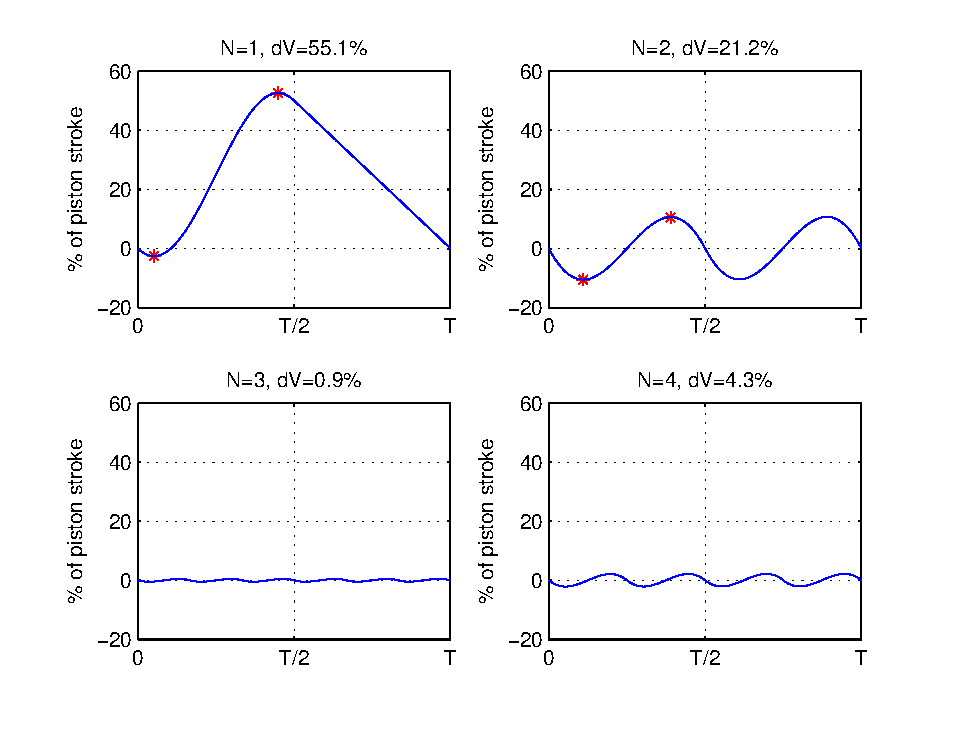
\includegraphics[width=0.8\textwidth]{piston_pumps}
\caption{\label{fig:pres_damp_volume}Volume change in the pressure dampener for different number of pistons.}
\end{center}
\end{figure}

Now let us find the pressure pulsation of the \emph{gas} due to the fluid volume change $\Delta V$. We start off by defining the pre-charge pressure $p_{pc}$ (e.g. 80\% of system pressure), at which the gas volume is $V_0$ (i.e. the nominal volume of the damper) and the required level of damping $\delta=(p_{max}-p_{min})/p_{sys}$. The corresponding \emph{gas} volumes will be $V_{max}$ (corresponding to $p_{min}$) and $V_{min}$ (corresponding to $p_{max}$). At system pressure, the the gas volume is $V_{sys}$. We also have $V^g_{max}=V^g_{min}+\Delta V$.

\noindent Notice that if the process is isotherm (which is usually true in real-life cases), we have)
%
\begin{equation}
\delta =\frac{p_{max}-p_{min}}{p_{sys}} = \frac{\Delta p}{p_{sys}} \approx\frac{\Delta V}{V_{sys}}
\end{equation}
%
\noindent We also have
%
\begin{equation}
p_{min}=p_{pc} \frac{V_0}{V_{max}}, \quad p_{sys}=p_{pc} \frac{V_0}{V_{sys}}\quad \text{and} \quad p_{max}=p_{pc} \frac{V_0}{V_{min}},
\end{equation}
%
and the pressure pulsation level is 
%
\begin{equation}
\delta =\frac{\Delta V}{V_{sys}} = \frac{\nu V_{stroke}}{V_0 \frac{p_{pc}}{p_{sys}}}
\label{eq:delta}
\end{equation}
%
hence the required dampener volume is
%
\begin{equation}
\shadowbox{$\displaystyle
V_0=\frac{\nu V_{stroke}}{\frac{p_{pc}}{p_{sys}} \delta}
$}
\end{equation}


\noindent {\bf Example.} We have a duplex pump ($N=2$, $\nu=0.2105$) with $s=60mm$ stroke and $D=63mm$ diameter.
%
\begin{itemize}
\item The stroke volume is $V_{stroke}=\frac{D^2 \pi}{4}s = 0.187$ liter
\item The precharge pressure is set to 80\% of system pressure: $p_{pc}/p_{sys}=0.8$
\item The required level of damping is $\delta=5\%$.
\item The nominal dampener volume is $V_0=\frac{0.2105 \times 0.187}{0.8\times 0.05}=0.984\approx1$ liter.
\end{itemize}

\clearpage


%%%%%%%%%%%%%%%%%%%%%%%%%%%%%%%%%%%%%%%%%%%%%%%%%%%%%%%%%%%%

\section{Pressure relief valves (PRV)}

As we have seen, the flow rate of a PDP is hardly affected by the system pressure, hence even if the flow rate need of the system is zero, the pump will convey the flow rate into the system. In such cases, the system pressure quickly rises and, if not vented, some component will break leading to a failure in the system. To prevent such problems, pressure relief valve (PRV) must are mounted {\bf as close to the pump as possible}.

These devices open above a \emph{set pressure} allowing controlled backflow to the the tank. If the system pressure is below the st pressure, the PRV remains closed and does not affect the system behaviour. There are two main types:
%
\begin{description}
\item[Direct spring loaded:] Usually used for low flow rate.
\item[Pilot operated:] High flow rate.
\end{description}

\subsection{Direct spring loaded hydraulic PRV}

Direct spring loaded pressure relief valves (DSLPRV) are simple and robust. The spool is balanced by a spring (upper side) and the pressure force (lower side). Note that the flow-through area varies with the valve lift (see Figures \ref{fig:direct_spring_loaded_PRV} and \ref{fig:detail_of_direct_spring_loaded_PRV}).

\begin{figure}[tbh]
\begin{center}
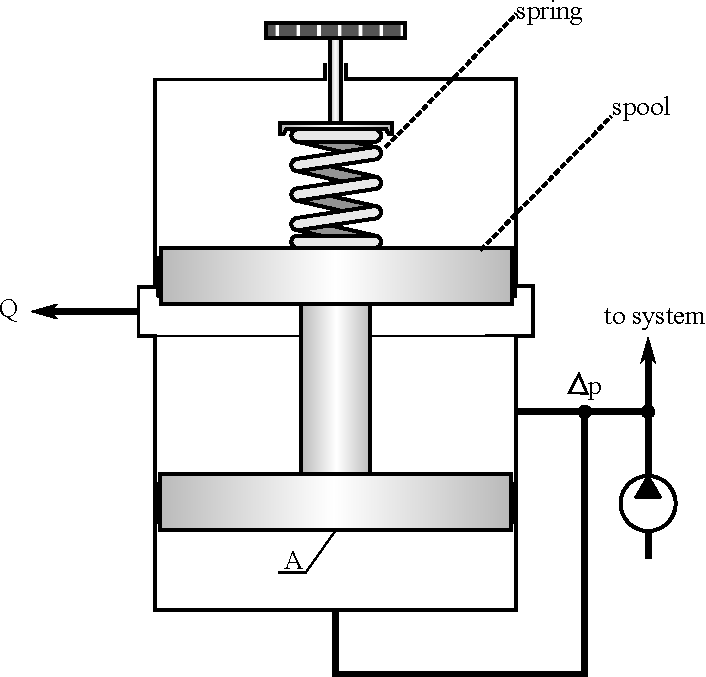
\includegraphics[scale=0.7]{lecture3_fig13a_dugattyus_szelep.pdf}
\caption{\label{fig:direct_spring_loaded_PRV}Direct spring loaded hydraulic PRV}
\end{center}

\end{figure}
\begin{figure}[tbh]
\begin{center}
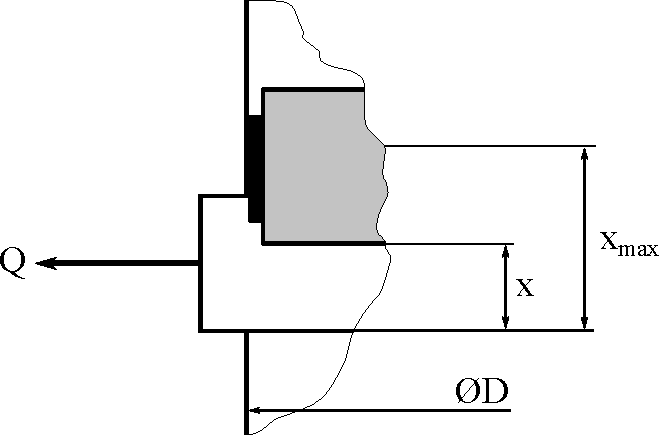
\includegraphics[scale=0.5]{lecture3_fig13b_dugattyus_szelep.pdf}
\caption{\label{fig:detail_of_direct_spring_loaded_PRV}Detail of a direct spring loaded hydraulic PRV}
\end{center}
\end{figure}

The force balance of the spool reads

\begin{equation}
s\left(x+x_{\mathrm{0}}\right)=A\Delta p.
\end{equation}

\noindent The \emph{set pressure}, at which the valve opens is given by $p_{set}=\frac{s x_0}{A}$. In general, the flow rate is $Q=C_d A_{ft}\sqrt{2 \Delta p/\rho}$. However, it should be noted that the flow-through area varies with the valve lift:
\begin{equation}
Q(\Delta p)=
\begin{cases}
0 & \mathrm{for} \quad x<0\\
C_{\mathrm{d}}A_{\mathrm{ft}}(x)\sqrt{\frac{2}{\rho}\Delta p}=C_{\mathrm{d}}D\pi \underbrace{\left( \frac{A\Delta p}{s}-x_0 \right)}_{x}\sqrt{\frac{2}{\rho}\Delta p} & \mathrm{for} \quad 0<x<x_{\mathrm{max}} \\
C_{\mathrm{d}}D\pi x_{\mathrm{max}}\sqrt{\frac{2}{\rho}\Delta p} & \mathrm{for} \quad x>x_{\mathrm{max}}
\end{cases}
\end{equation}

Note that in the middle range, we have
\begin{equation}
Q(\Delta p)=
C_d D \pi\frac{A}{s} \sqrt{\frac{2}{\rho}} \left( \Delta p - \frac{x_0 s}{A}\right)\sqrt{\Delta p} \propto \left( \Delta p - p_{set}\right)\sqrt{\Delta p},
\end{equation}
%
that is, it is zero if $\Delta p=0$ and $\Delta p =p_{set}$. Moreover, for $0\leq\Delta p \leq p_{set}$ this function is negative, for $\Delta p>p_{set}$, the flow rate is proportional to $\Delta p^{3/2}$. The actual plot is shown in Figure \ref{fig:direct_spring_loaded_PRV_inverse_curve}.


\begin{figure}[tbh]
\begin{center}
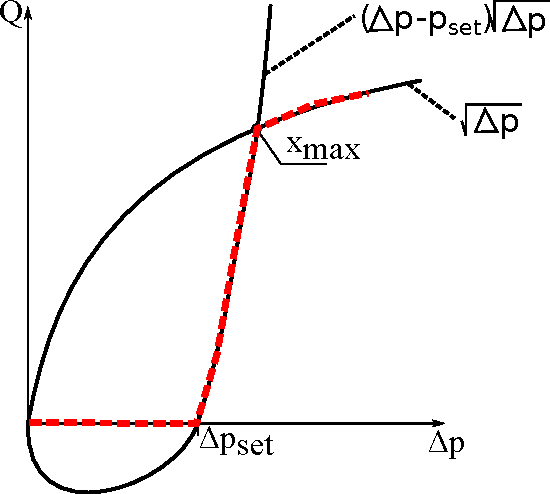
\includegraphics[scale=0.8]{lecture3_fig14_dugattyus_szelep_dp_Q.pdf}
\caption{\label{fig:direct_spring_loaded_PRV_Q(dp)}$Q(\Delta p)$ curve of a direct spring loaded hydraulic PRV}
\end{center}
\end{figure}
$\Delta p$ in normal operation: $\Delta p\cdot \sqrt{\Delta p}=\Delta p^{3/2}$ $\rightarrow$ it is between $\Delta p\dots \Delta p^{3/2}\dots \Delta p^2$
The usual way of plotting the characteristic curve is inverse (also in catalogue):
\begin{figure}[tbh]
\begin{center}
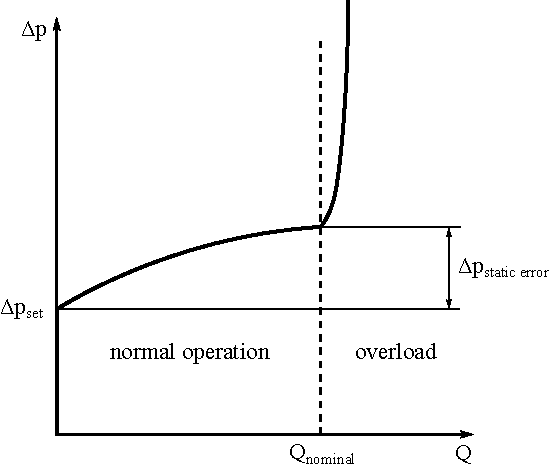
\includegraphics[scale=0.8]{lecture3_fig15_dugattyus_szelep_dp_Q_inverz.pdf}
\caption{\label{fig:direct_spring_loaded_PRV_inverse_curve}Inverse $Q(\Delta p)$ curve of a direct spring loaded hydraulic PRV}
\end{center}
\end{figure}
Note: $\Delta p_{\mathrm{static}}\approx (0.01\dots 0.1)\Delta p_{\mathrm{set}}$.
\subsubsection{Dynamic error}
When it opens quickly.
\begin{figure}[tbh]
\begin{center}
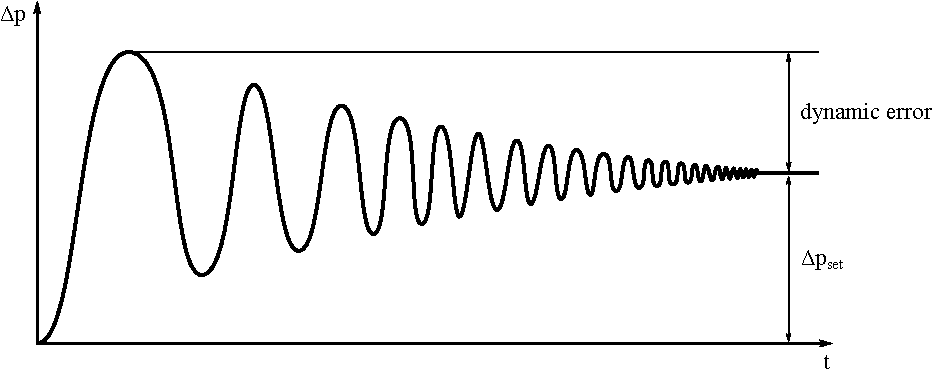
\includegraphics[width=100mm]{lecture3_fig16_dugattyus_szelep_dinamikus_hiba.pdf}
\caption{\label{fig:dynamic_error_of_direct_spring_loaded_PRV}Dynamic error of a direct spring loaded hydraulic PRV}
\end{center}
\end{figure}
Note: $\Delta p_{\mathrm{dyn}}$ can be $2\dots 3$ times bigger than $\Delta p_{\mathrm{set}}$.
\subsubsection{Sizing of a pressure relief valve}
\begin{equation}
Q_{\mathrm{pump,max}}<Q_{\mathrm{PRV,max}}
\end{equation}

\begin{figure}[tbh]
\begin{center}
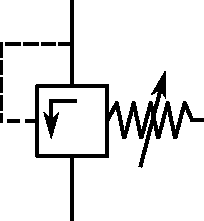
\includegraphics[scale=1]{lecture3_fig17b_biztonsagi_szelep.pdf}
\caption{\label{fig:PRV}Standard symbol of PRV}
\end{center}
\end{figure}

\subsubsection{Examples}
\paragraph{Hydraulic aggregate}
Pump and PRV.
\begin{figure}[tbh]
\begin{center}
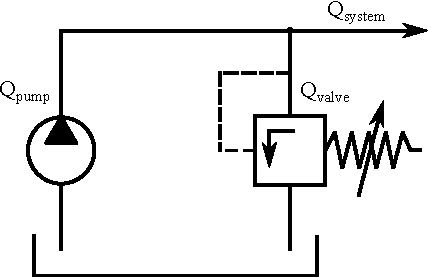
\includegraphics[scale=0.8]{lecture3_fig17a_biztonsagi_szelepes_rendszer.pdf}
\caption{\label{fig:hydraulic_aggregate}Hydraulic aggregate}
\end{center}
\end{figure}
\begin{figure}[tbh]
\begin{center}
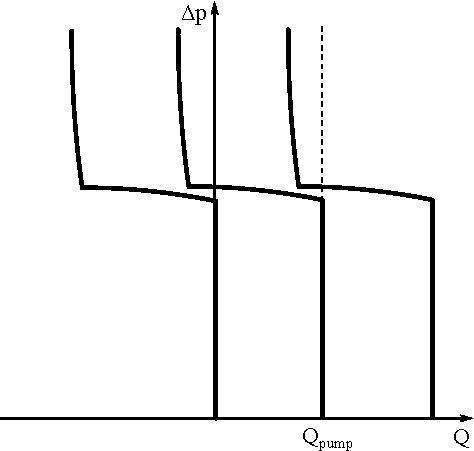
\includegraphics[scale=0.8]{lecture3_fig18_biztonsagi_szelepes_rendszer_Q_dp.pdf}
\caption{\label{fig:?}\fbox{19 caption}}
\end{center}
\end{figure}\begin{figure}[tbh]
\begin{center}
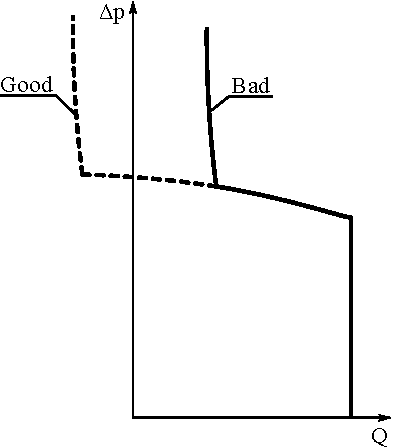
\includegraphics[scale=1]{lecture3_fig19_biztonsagi_szelepes_rendszer_Q_dp_helyes_hibas.pdf}
\caption{\label{fig:??}\fbox{20 caption}}
\end{center}
\end{figure}
\paragraph{In gas systems}
Natural gas industry.
\begin{figure}[tbh]
\begin{center}
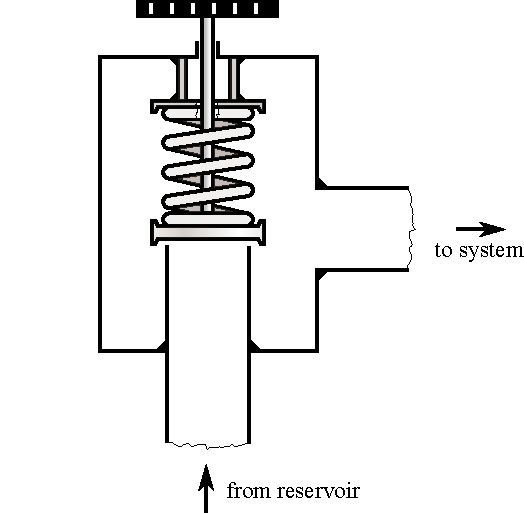
\includegraphics[scale=0.8]{lecture3_fig20_foldgaz_szelep.pdf}
\caption{\label{fig:PRV_gas_industry}PRV used in natural gas industry}
\end{center}
\end{figure}


\clearpage

\subsection{Pilot operated pressure relief valve}
As $Q_{\mathrm{nominal}}$ increases, the static error also increases.
\begin{figure}[tbh]
\begin{center}
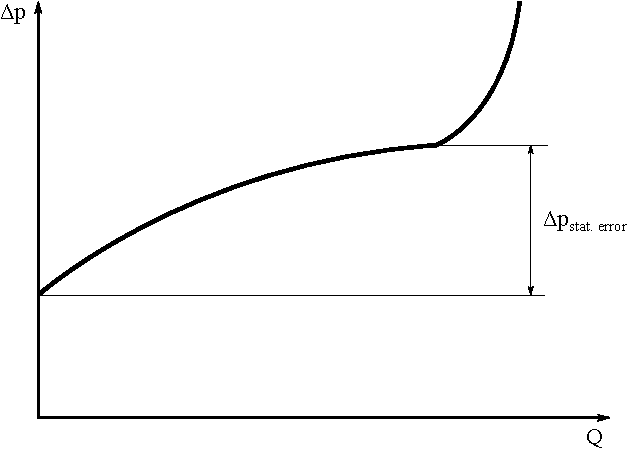
\includegraphics[scale=0.8]{lecture3_fig21_szelep_statikus_hiba.pdf}
\caption{\label{fig:static_error_of_PRV}Static error of a direct spring loaded PRV}
\end{center}
\end{figure}
In this case we can use pilot operated PRV.
\begin{equation}
Q=C_{\mathrm{d}}D\pi\left(\frac{A\Delta p}{s}-x_{\mathrm{0}}\right)\sqrt{\frac{2}{\rho}\Delta p}
\end{equation}
\begin{tabbing}
Let \=$Q_{\mathrm{nominal}}$ be given: $Q$ at $\Delta p_{\mathrm{max}}$ \\
\> $\Delta p_{\mathrm{set}}$ be given: $\Delta p_{\mathrm{set}}=\frac{sx_{\mathrm{0}}}{A}$
\end{tabbing}
If higher flow rate is needed: increase $D$.
\begin{equation}
\frac{sx_{\mathrm{0}}}{A}=\frac{sx_{\mathrm{0}}}{\frac{D^2\pi}{4}}=\Delta p_{\mathrm{set}}
\end{equation}
Increase $s$ (stiffer spring)) or $x_{\mathrm{0}}$ (higher precompression) to keep $\Delta p_{\mathrm{set}}$ as constant value.

However the slope of the curve in the normal operation:
\begin{equation}
\frac{\mathrm{d}}{\mathrm{d}\Delta p}Q=\frac{\mathrm{d}}{\mathrm{d}\Delta p}\left(C_{\mathrm{d}}D\pi\left(\frac{D^2\pi}{\frac{4}{s}}\right)\sqrt{\frac{2}{\rho}}\Delta p^{3/2}\right)\sim \frac{D^3}{s}\frac{3}{2}\sqrt{\Delta p}
\end{equation}
and $s \sim D^2$.
\paragraph{1st choise}
Let $s \sim D^2$. $\Delta p_{\mathrm{set}}=\frac{sx_{\mathrm{0}}}{\frac{D^2\pi}{4}}$ remains constant.
Slope $\sim$ static error $\sim$ D.
\paragraph{2nd choise}
$s$ is constant $x_{\mathrm{0}} \sim D^2 \rightarrow \mathrm{slope} \sim D^3$.
Too high static error! Solution: pilot operated PRV.

\begin{figure}
\begin{center}
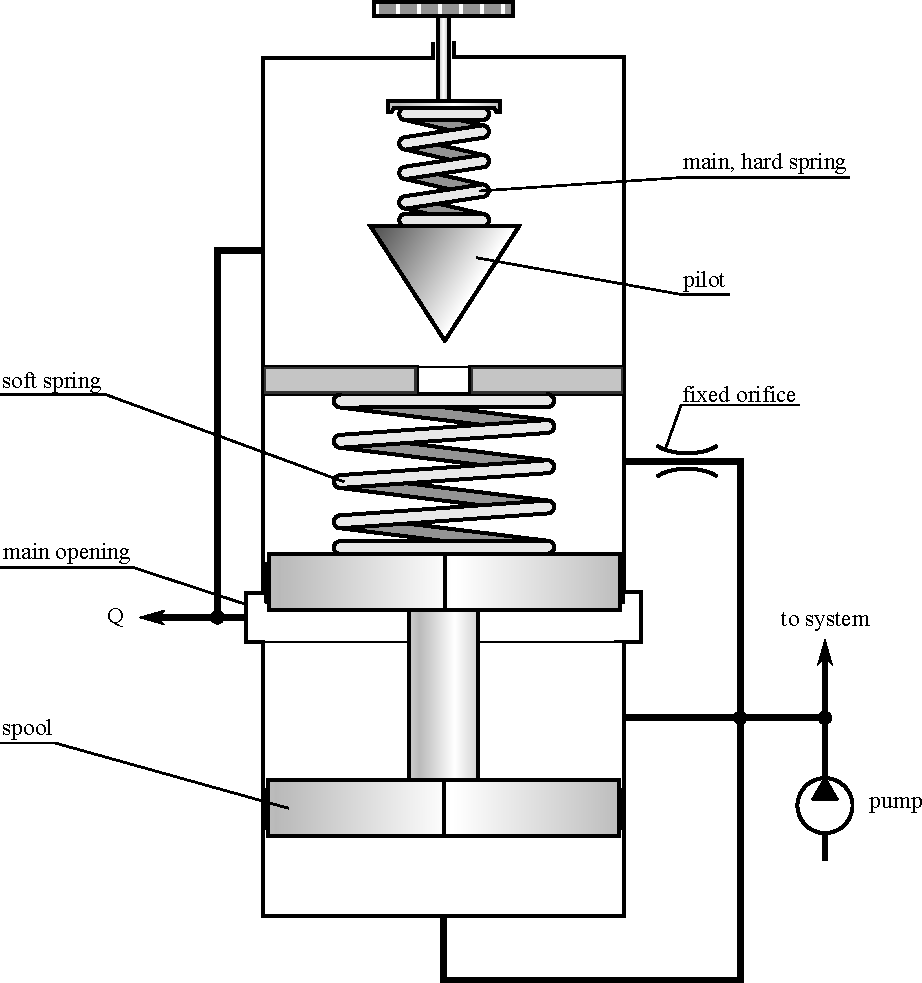
\includegraphics[scale=0.5]{lecture3_fig22_dugattyus_szelep_ket_rugos.pdf}
\caption{\label{fig:pilot_operated_PRV}Pilot operated PRV}
\end{center}
\end{figure}

\subsubsection{Operating progress of the valve}
Pressure drops because of the fixed orifice $\rightarrow$ the spool moves upwards $\rightarrow$ it opens the main opening.
\subsubsection{Important details}
\begin{itemize}
\item[--] Right location of the soft and hard springs
\item[--] Fixed orifice
\end{itemize}
\section{Sizing of simple hydraulic systems}

\clearpage

\subsection{System with motor}

\begin{figure}[tbh]
\begin{center}
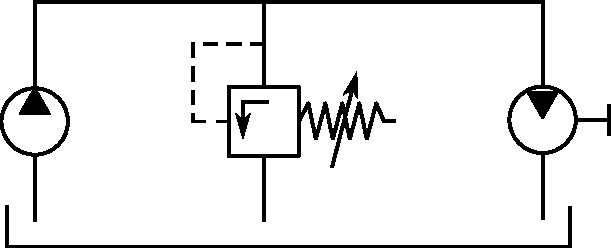
\includegraphics[scale=0.8]{lecture4_fig23_szivattyus_motoros_rendszer.pdf}
\caption{\label{fig:hydraulic_aggregate_with_motor}Hydraulic aggregate with motor}
\end{center}
\end{figure}

User data: $M_{\mathrm{motor}}$, $n_{\mathrm{motor}}$\\
Sizing: $V_{\mathrm{g,pump}}$, $p_{\mathrm{set}}$, $V_{\mathrm{g,motor}}$, control
\subsubsection{Example for a system with motor}
$M_{\mathrm{motor}}=100\,\mathrm{Nm}$, $n_{\mathrm{motor}}=1500\,\mathrm{rpm}$
\paragraph{Motor}
\begin{equation}
Q\Delta p \eta_{\mathrm{hm}}=M2\pi n
\end{equation}
$\Delta p \sim M$ and $Q \sim n$ $\rightarrow $ $V_{\mathrm{g}}$\\
From catalogue: $\Delta p=280\,\mathrm{bar}$ $\rightarrow$ size: 23 $\rightarrow$ $M_{\mathrm{motor}}=105\,\mathrm{Nm}$ and $V_{\mathrm{g}}=23.5\,\mathrm{cm^3}$
\begin{equation}
Q_{\mathrm{motor}}=V_{\mathrm{g}}n_{\mathrm{motor}}=23.5\times 10^{-3}\,\mathrm{l/min}\times 1.5\times 10^{3}\,\mathrm{1/min}=35.25\,\mathrm{l/min}
\end{equation}
Output of the sizing: $\Delta p$, $Q$. In this calculation $\eta \cong 1$.
\subsection{System with cylinder}

\begin{figure}[tbh]
\begin{center}
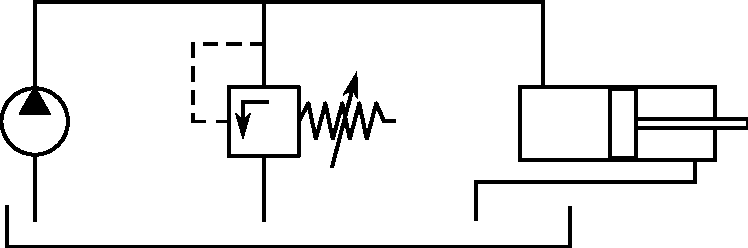
\includegraphics[scale=0.8]{lecture4_fig24_szivattyus_munkahengeres_rendszer.pdf}
\caption{\label{fig:hydraulic_aggregate_with_cylinder}Hydraulic aggregate with cylinder}
\end{center}
\end{figure}
User data: $F$, $v$\\
Sizing: $V_{\mathrm{g,pump}}$, $p_{\mathrm{set}}$, $\frac{D}{d}$, control
\paragraph{Piston control valve}

\begin{figure}[tbh]
\begin{center}
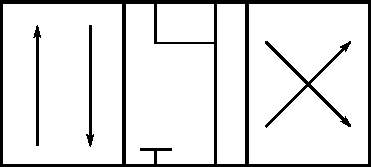
\includegraphics[scale=0.6]{lecture4_fig25_utirany_szelep.pdf}
\caption{\label{fig:piston_control_valve}Symbol of the piston control valve}
\end{center}
\end{figure}
\begin{figure}[tbh]
\begin{center}
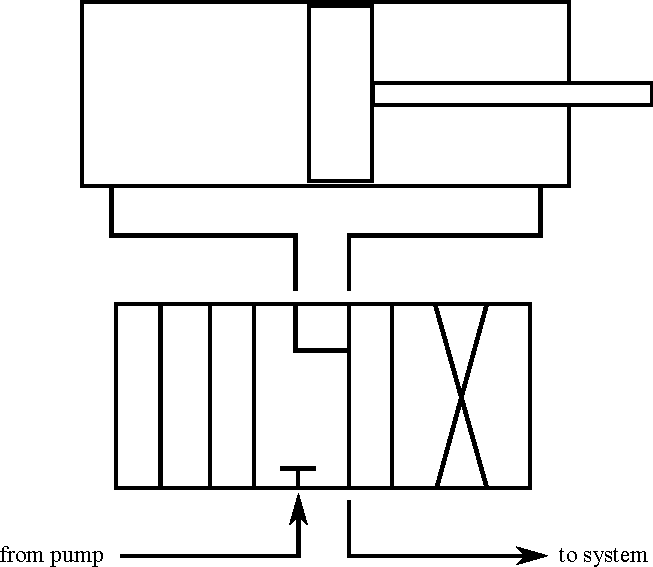
\includegraphics[scale=0.5]{lecture4_fig26_utirany_szelep_munkahengerrel.pdf}
\caption{\label{fig:piston_control_valve_with_cylinder}Piston control valve with cylinder}
\end{center}
\end{figure}

From catalogue: $V_{\mathrm{g,pump}}$, $V_{\mathrm{g,motor}}$, $\frac{D}{d}$
\subsubsection{Example for a system with cylinder}
$M_{\mathrm{motor}}=100\,\mathrm{Nm}$, $n_{\mathrm{motor}}=1500\,\mathrm{rpm}$
\begin{equation}
nV_{\mathrm{g}}\Delta p=M2\pi n
\end{equation}
\begin{equation}
\Delta p=\frac{M2\pi n}{n V_{\mathrm{g}}}=\frac{2\pi M}{V_{\mathrm{g}}}=\frac{2\pi 100}{V_{\mathrm{g}}}=\frac{2\pi 100}{28.5\times10^{-6}}=220\,\mathrm{bar}
\end{equation}
\begin{equation}
Q={V_{\mathrm{g}}}n_{\mathrm{motor}}=28.5\times 1.5=42.75\,\mathrm{l/min}
\end{equation}
Pick size 28. The aggregate should provide this flow rate at the $\Delta p$ pressure.
\paragraph{Pump}
Driving motor speed: $n_{\mathrm{pump}}=3000\,\mathrm{rpm}$
\begin{equation}
Q_{\mathrm{pump}}=n_{\mathrm{pump}}V_{\mathrm{g,pump}}\rightarrow V_{\mathrm{g,pump}}=\frac{Q_{\mathrm{pump}}}{n_{\mathrm{pump}}}=\frac{28.5\,\mathrm{l/min}}{3000\,\mathrm{rpm}}=14.25\,{\mathrm{cm^3}}
\end{equation}
Pick $V_{\mathrm{g,pump}}=16\,{\mathrm{cm^3}}$.
With the new value:
\begin{equation}
Q_{\mathrm{pump}}=n_{\mathrm{pump}}V_{\mathrm{g,pump}}=3000\,\mathrm{rpm}\times 16\,\mathrm{cm^3}=48\,\mathrm{l/min}
\end{equation}
\paragraph{Set pressure of the PRV}
$120\,\mathrm{\%}$ of the highest expected system pressure.
\begin{equation}
p_{\mathrm{set}}:=1.2\times 220=264\,\mathrm{bar}
\end{equation}
$Q_{\mathrm{nom,PRV}}>42.8\,\mathrm{l/min}\ \mathrm{(capacity\ of\ PRV)}$.
\subsection{Control techniques}
\begin{itemize}
\item[--] Throttle valve in parallel connection
\item[--] Throttle valve in series connection
\item[--] Frequency converter
\item[--] Special pump: variable displacement motor, variable $V_{\mathrm{g}}$
\item[--] Motor speeed $(n)$ changing
\end{itemize}
\subsubsection{Throttle valve in parallel connection}
\begin{figure}[tbh]
\begin{center}
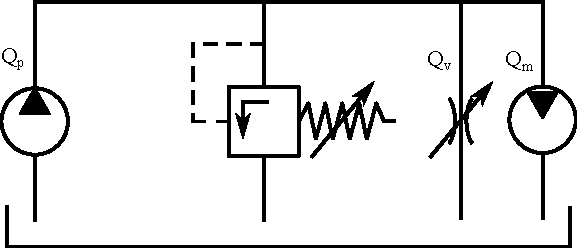
\includegraphics[scale=0.8]{lecture4_fig27_szivattyus_motoros_rendszer_parhuzamos_fojtas.pdf}
\caption{\label{fig:throttle_valve_parallel}System with throttle valve in parallel connection}
\end{center}
\end{figure}
$\Delta p$ is the same. PRV is closed.

\subsubsection{Throttle valve in series connection}
\begin{figure}[tbh]
\begin{center}
\includegraphics[scale=0.8]{lecture4_fig28_szivattyus_motoros_rendszer_soros_fojtas.pdf}
\caption{\label{fig:throttle_valve_series}System with throttle valve in series connection}
\end{center}
\end{figure}
$Q$ is the same. PRV is open.

%\input{pressure_vessel_sizing.tex}


% In gear pumps the liquid is trapped by the opening between the gear teeth of two identical gears and the chasing of the pump on the suction side. On the pressure side the fluid is squeezed out when the teeth of the two gears are rotated against each other. The motor provides the drive for one gear.

% The lobe pumps operates similar to the gear pump, but with two lobes driven by external timing gears. The lobes do not make contact.

% Progressive cavity pumps consist of a metal rotor rotating within an elastomer-lined or elastic stator. When the rotor turns progressive chambers from suction end to discharge end are formed between the rotor and stator, moving the fluid. 


\section{Problems}

\noindent {\bf Problem \thesection.\theprob}\stepcounter{prob}

Calculate the hydraulic power of the double-acting piston pump, which delivers water from an open-surface tank into a closed one with $500[kPa]$ gauge pressure (i.e. relative pressure) located $50[m]$ above the suction tank. Diameter of the piston is $D=120[mm]$, the stroke is $150[mm]$ and the driving motor runs at $120[rpm]$.

\emph{Solution:} 

$Q_{mean}=2 \times A_{piston} \times s \times n=2\times \frac{0.12^2 \pi}{4} \times 0.15 \times \frac{120}{60} =6.78 \times 10^{-3} [\frac{m^3}{s}]$

$\Delta p=p_{tank,abs.}-p_0\,+\,\rho g H=p_{tank,rel.}\,+\,\rho g H=991[kPa]$

$P=Q \Delta p=6.72[kW]$

%%%%%%%%%%%%%%%%%%%%%%%%%%%%%%%%%%%%%%%%%%%%%%%%%%%%

\vspace{1cm}
\noindent {\bf Problem \thesection.\theprob}\stepcounter{prob}

The characteristic curve of a gear pump is $Q[dm^3/min]=11.93-0.0043 \Delta p [bar]$. The volumetric efficiency at $35 bar$ pressure difference is $92\%$. Find the volume flow rate and the geometric volume! The shaft speed is $80 rev/min$. How large is the driving torque if the pump efficiency is $85\%$? (Solution: $Q=11.78\,dm^3/min$, $V_g = 160\,cm^3$, $M = 96.5\,Nm$)

%%%%%%%%%%%%%%%%%%%%%%%%%%%%%%%%%%%%%%%%%%%%%%%%%%%%

\vspace{1cm}
\noindent {\bf Problem \thesection.\theprob}\stepcounter{prob}

The piston diameter of a hydraulic cylinder is $50 mm$. An $800 kg$ load is lifted by the piston rod of $20 mm$ diameter with $12 m/min$ velocity. How large must be the flow rate $Q$ of the gear pump rotating with $n = 960/min$ speed if its volumetric efficiency is $92\%$? Find the geometric volume of the pump and the pressure rise produced by it! Find the power $P$ and the torque $M$ of the driving motor! The pump efficiency is $74\%$. Prepare a sketch of the gear pump showing the rotation direction of the shafts, intake and delivery ports! How large will be $P’$, $M$, $Q’$ if the rotor speed is $n’ = 1440/min$? (Solution: $Q_g = 21.5\,dm^3/min$, $V_g = 22.4\,cm^3$, $\Delta p = 47.6\,bar$, $P=2.12\,kW$, $M=21.1\,Nm$, $P_{1440}=3.18\,kW$, $Q_{1440} = 32.25\,dm^3/min$, $M_{1440}=21.1\,Nm$)

%%%%%%%%%%%%%%%%%%%%%%%%%%%%%%%%%%%%%%%%%%%%%%%%%%%%

\vspace{1cm}
\noindent {\bf Problem \thesection.\theprob}\stepcounter{prob}

The piston diameter of a vertical hydraulic cylinder is supporting a mass of $700 kg$. It may not be lowered faster than $64 mm/s$. The cylinder diameter is $50 mm$, the piston rod diameter is $28 mm$. The pump delivery curve is $Q [liter/min] = 8.6-0.0467 \Delta p[bar]$. The hydraulic oil of $970 kg/m^3$ density leaves the cylinder through a throttle valve. The discharge coefficient of this valve is $\mu=0.7$. Find the valve area at the maximal opening! Find the maximum of the useful power of the pump! 

Solution:

\begin{wrapfigure}{R}{0.4\textwidth}
\includegraphics[width=0.4\textwidth]{Problem_solving/figs/cylinder-problem.png}
\end{wrapfigure}

The two areas:
\begin{align*}
A_{ring} = \frac{\pi}{4} (D^2-d^2) = 0.001348~\mathrm{m^2}\\
A = \frac{\pi}{4} D^2 = 0.001964~\mathrm{m^2}.
\end{align*}

Newton's law:
%\begin{align*}
%A(p_0+\Delta p_{valve}) = A_{ring}p + mg = A_{ring}(p_0 + \Delta p) + mg + A_{piston}p_0 = Ap_0 + A_{ring} \Delta p + mg.
%\end{align*}
\begin{multline*}
A(p_0+\Delta p_{valve}) = A_{ring}p + mg = \\
A_{ring}(p_0 + \Delta p) + mg + A_{piston}p_0 = Ap_0 + A_{ring} \Delta p + mg.
\end{multline*}

Continuity equation for the upper part of the cylinder:
\begin{align*}
Q_{pump} = A_{ring}v = 0.001347~\mathrm{m^2}\cdot 0.064~\frac{\mathrm{m}}{\mathrm{s}} = 5.176~\frac{\mathrm{dm^3}}{\mathrm{min}}.
\end{align*}

Pressure from the performance curve of the pump:
\begin{align*}
\Delta p = \frac{8.6-Q_{pump}}{0.0467} = \frac{8.6-5.176}{0.0467} = 73.3~\mathrm{bar}.
\end{align*}

Continuity equation for the valve:
\begin{align*}
Q_{valve} = Av = 0.001964~\mathrm{m^2}\cdot 0.064~\frac{\mathrm{m}}{\mathrm{s}} = 7.54~\frac{\mathrm{dm^3}}{\mathrm{min}}.
\end{align*}

Bernoulli's equation for the valve: 
\begin{align*}
Q_{valve} = \mu A_{valve}\sqrt{\frac{2}{\rho_{oil}}\Delta p_{valve}}.
\end{align*}

Rearranging Newton's law yields
\begin{align*}
\Delta p_{valve} = \frac{A_{ring}\Delta p + mg}{A} = \frac{0.001348\cdot 7.33\cdot 10^6 + 700\cdot 9.81}{0.001964} = 85.27~\mathrm{bar}, 
\end{align*}
and finally,
\begin{align*}
A_{valve} = \frac{Q_{valve}}{\mu \sqrt{\frac{2}{\rho_{oil}}\Delta p_{valve}}} = \frac{0.0001257}{0.7\cdot \sqrt{\frac{2}{970}\cdot 85.27\cdot 10^5}} = 1.354~\mathrm{mm}.
\end{align*}

The useful power of the pump is
\begin{align*}
P_{p,u}=Q_{pump}\Delta p_{pump} = (8.6-0.0467 \Delta p)\Delta p.
\end{align*}

The criterion for the local maximum is $\frac{\mathrm{d}P_{p,u}}{\mathrm{d}\Delta p} = 8.6-2\cdot 0.0467\cdot \Delta p_{opt} = 0 \rightarrow \Delta p_{opt} = 92.1~\mathrm{bar}$. At this operating point, $Q_{opt}=4.3~\frac{1}{\mathrm{min}}$, and $P_{p,u,max} = 660~\mathrm{W}$.


\clearpage

%\section{Problems}

%\noindent {\bf Problem \thesection.\theprob}\stepcounter{prob}

%Calculate the hydraulic power of the double-acting piston pump, which delivers water from an open-surface tank into a closed one with $500[kPa]$ gauge pressure (i.e. relative pressure) located $50[m]$ above the suction tank. Diameter of the piston is $D=120[mm]$, the stroke is $150[mm]$ and the driving motor runs at $120[rpm]$.

%\emph{Solution:} 

%\begin{itemize}
%\item $Q_{mean}=2 \cdot A_{piston} \cdot s \cdot n=2\cdot \frac{0.12^2 \pi}{4} \cdot 0.15 \cdot \frac{120}{60} =6.78 \cdot 10^{-3} [\frac{m^3}{s}]$
%\item $\Delta p=p_{tank,abs.}-p_0\,+\,\rho g H=p_{tank,rel.}\,+\,\rho g H=991[kPa]$
%\item $P=Q \Delta p=6.72[kW]$
%\end{itemize}
